\documentclass[12pt,a4paper]{article}

% Essential packages for robust design
\usepackage[utf8]{inputenc}
\usepackage[T1]{fontenc}
\usepackage{amsmath,amssymb,amsthm}
\usepackage{mathtools}
\usepackage[margin=1in]{geometry}
\usepackage{microtype}
\usepackage{hyperref}
\usepackage{cleveref}
\usepackage{graphicx}
\usepackage{tikz}
\usepackage{booktabs}
\usepackage{enumitem}
\usepackage[numbers,sort&compress]{natbib}

% Theorem environments
\newtheorem{theorem}{Theorem}[section]
\newtheorem{lemma}[theorem]{Lemma}
\newtheorem{proposition}[theorem]{Proposition}
\newtheorem{corollary}[theorem]{Corollary}
\theoremstyle{definition}
\newtheorem{definition}[theorem]{Definition}
\newtheorem{example}[theorem]{Example}
\theoremstyle{remark}
\newtheorem{remark}[theorem]{Remark}

% Hyperref setup
\hypersetup{
    colorlinks=true,
    linkcolor=blue,
    filecolor=magenta,      
    urlcolor=cyan,
    citecolor=blue,
    pdftitle={Quantum Coherence as Gated Recognition},
    pdfauthor={Author Name},
}

\title{Quantum Coherence as Gated Recognition: \\ 
An Eight-Tick Mechanism with Parameter-Free Bridges}

\author{Jonathan Washburn\thanks{Recognition Physics Email: \texttt{washburn@recognitionphysics.org}} \\
\textit{Recognition Physics Institute}}

\date{\today}

\begin{document}

\maketitle

\begin{abstract}
We address the core question of \emph{quantum coherence}: when is phase information preserved and when does it dephase under realistic readout? We show that coherence is an operational property of a discrete recognition process obeying exact eight-tick window identities. These identities provide necessary and sufficient conditions for phase preservation over aligned windows and act as a matched filter that retains only structure aligned to the eight-tick schedule while canceling everything else.

Quantitatively, a unique convex, multiplicatively symmetric cost on $\mathbb{R}_{>0}$,
\begin{equation}
J(x) = \tfrac{1}{2}(x + x^{-1}) - 1,\qquad J(e^t)=\cosh t - 1,
\end{equation}
is characterized by symmetry, unit normalization, and a Jensen-type averaging principle on the log axis. From $J$ we build a path weight that yields the Born rule (modulus) and, via permutation invariance, the BE/FD exchange classes. Together with atomicity and exactness (discrete $w=\nabla\phi$), the eight-tick schedule stabilizes coarse phase and quantifies when interference survives averaging.

We give operational audits and predictions: (i) exact window-8 sum/average equalities; (ii) a matched-filter coherence theorem with a phase-drift bound; (iii) multi-probe scaling laws (logarithmic extension of visible coherence time), (iv) discrete-lag cosines with a stretched-exponential envelope, and (v) a units K-gate consistency check for display ratios. All statements are presented in classical notation and are accompanied by mechanized witnesses (Lean) and a minimal audit manifest.

\noindent\textbf{Keywords:} quantum coherence, eight-tick schedule, matched filter, Born rule, BE/FD symmetrization, formal verification

\noindent\textbf{MSC 2020:} 81P15, 81P40, 03B35
\end{abstract}

\section{Introduction}

The standard account of quantum mechanics treats \emph{measurement} as a special operation requiring additional postulates. This paper develops a simpler alternative: \emph{measurement is recognition}. We formalize recognition as a discrete, ledger-like process that renders observation an explicit operation with cost and invariants. Within this framing, coherence emerges as a bookkeeping condition rather than a dynamical mystery; classical appearance is an averaging effect rather than an ontological add-on; and the usual probability rule arises from a single, symmetry‑and‑averaging constrained cost functional. Along the way, we connect the discrete ledger to a continuum via a coarse‑grained bridge, identify a canonical recognition length from anchors $(G,\hbar,c)$, and show how units, scales, and dimensionless gates fit together coherently.

All claims that follow are checked by machine. The theory is implemented in a proof assistant and compiled into a set of public, automated certificates \\
(e.g., \texttt{path\_cost\_isomorphism\_report}, \texttt{certificates\_manifest}) that accompany this paper.

\subsection{Motivation: coherence without added postulates (measurement as recognition)}
\label{sec:motivation}

The empirical \emph{weirdness} of measurement evaporates if we refuse to smuggle its cost and structure into the dynamics for free. In our approach:
\begin{itemize}
  \item A \emph{recognition structure} is a finite ledger of postings (events) indexed by atomic ticks, with a unique-posting invariant at each tick. Atomicity guarantees that no two outcomes are posted at the same tick (\emph{no collision}); conservation of closed flux guarantees that consistent ledgers remain consistent when spliced. Formally, these appear as: (i) a per-tick uniqueness property (\emph{T2: Atomicity}) and (ii) a closed-chain continuity property (\emph{T3: Conservation}) on the ledger chain.
  \item \emph{Coherence} is the statement that recognitions stitched across a small, fixed microcycle remain jointly satisfiable. Empirically we find an eight‑tick microcycle to be the minimal stable unit for policy‑invariant recognition (``eight‑tick coherence''): it is the smallest window in which the ledger can enforce timeliness, reciprocity, and temperance simultaneously while maintaining unique postings and closed flux.%
  \footnote{Eight‑tick coherence is the operational window in which the recognition gates are jointly satisfiable without contradiction; in later sections we connect this to arithmetic constraints (the $8 \leftrightarrow 45$ interference window) and to coarse‑grained continuum limits.}
  \item \emph{Measurement} is therefore nothing more than a particular recognition protocol over this ledger: which postings are permitted, when they are permitted (ticks), and which equivalences are quotiented away by coarse views (averaging).
\end{itemize}

In this view, the notorious ``measurement postulate'' is replaced by a concrete, auditable protocol: a recognition rule with invariants, a microcycle scale (eight ticks), and explicit averaging (Section~\ref{sec:prior-art-as-recognition}). This shift reduces interpretational load while strengthening predictive structure: any phenomenon explainable as ``collapse'' becomes a statement about which recognitions are admissible and at what cost.

\subsection{Prior art reframed as recognition/averaging}
\label{sec:prior-art-as-recognition}

The path integral, decoherence, and coarse‑graining programs are typically presented as formal machinery layered on quantum states. We re-express each as recognition/averaging primitives inside the ledger.

\paragraph{Path integrals as recognition sums.}
Sum‑over‑histories can be recast as a \emph{recognition sum} over ledger chains. Each candidate chain $\,\gamma\,$ is a sequence of postings satisfying the atomicity and continuity constraints; amplitudes assign complex weights to these chains. Recognition does not require adding collapse rules: selecting an outcome corresponds to choosing an equivalence class of chains (same recognitions up to gauge on constants), and \emph{averaging} is the natural coarse view that forgets ledger‑exact details outside the eight‑tick window. The phase structure remains in the recognizer through relative costs (see below), while the act of reading an outcome is just ``which chain class did the policy admit?''

\paragraph{Decoherence as admissibility filtering.}
Traditional decoherence formalizes the suppression of interference terms by tracing over environments. In a recognition ledger, this is rephrased as \emph{admissibility filtering}: the gates that enforce timeliness, reciprocity, and temperance on eight‑tick windows forbid many fine‑grained postings (they cannot be jointly posted without violating atomicity or closed‑flux). The resulting \emph{block‑diagonalization} is simply the set of recognitions that survive the policy at bounded cost, i.e., those that remain jointly satisfiable under averaging over the unobserved dofs.

\paragraph{Coarse‑graining as Riemann recognition.}
Passing to a continuum description is not metaphysics; it is a limit of recognition sums. A coarse‑graining schema maps ticks to cells with positive volumes and defines Riemann sums for observables over embedded cells. In the limit, discrete conservation laws pass to a divergence form continuity equation. This provides a precise bridge: the continuum PDEs we solve are statements about the limit of recognitions of conserved ledger flux under averaging.

\subsection{This work: discrete ledger $\to$ eight‑tick coherence, unique cost $\to$ Born, audits $\to$ units}
\label{sec:this-work}

This paper contributes three pieces that, together, turn \emph{measurement as recognition} into a predictive, auditably coherent framework.

\paragraph{(A) Discrete ledger $\to$ eight‑tick coherence.}
We present a recognition ledger with:
\begin{enumerate}
  \item \textbf{Atomic ticks} (\emph{T2}): a uniqueness guarantee that exactly one posting is recognized per tick.
  \item \textbf{Closed‑flux continuity} (\emph{T3}): any closed chain of postings conserves its net ledger flux; chains that begin and end at the same state have zero net flux.
  \item \textbf{Eight‑tick microcycles}: the minimal window in which timeliness (no late postings), reciprocity (no stakeholder imbalance), and temperance (bounded magnitudes) are jointly satisfiable \emph{and} compatible with T2/T3. We justify eight as the minimal stable coherence window and characterize how larger windows factor through concatenations of eight‑tick microcycles.
\end{enumerate}
These ingredients are enough to reproduce the qualitative content of decoherence and to support a coarse‑grained bridge to continuum dynamics without auxiliary postulates.

\paragraph{(B) Unique cost $\to$ Born.}
At the heart of recognition is a convex averaging on the log‑axis that quantifies the \emph{cost} of reconciling candidate recognitions. Symmetry (invariance under $x \mapsto x^{-1}$), unit normalization, and Jensen‑type averaging on the exponential axis uniquely determine the cost functional
\[
  J(x) \;=\; \frac{x + x^{-1}}{2} - 1,
  \qquad
  \text{equivalently}\quad J(\mathrm{e}^t) \;=\; \cosh t - 1,
\]
and we prove that any $F$ satisfying the symmetry/unit axioms and the averaging bounds agrees with $J$ on $\mathbb{R}_{>0}$. In recognition terms: $J$ is the \emph{only} admissible distortion measure compatible with the invariants of measurement-as-recognition.

The Born rule then follows as the unique recognition‑consistent weighting. Squared amplitudes appear as the only weights for which (i) eight‑tick coherence is preserved under admissibility filtering, (ii) costs aggregate additively under coarse‑graining, and (iii) the recognition probabilities are stable under refinement (no Dutch book across concatenated microcycles). Thus, what is often introduced as an additional axiom is, here, the only fixed point of the recognition cost calculus.

\paragraph{(C) Audits $\to$ units.}
Finally, we exhibit a minimalist audit that converts recognition ticks and lengths into display ratios without extra structure. Two ingredients are sufficient:
\begin{enumerate}
  \item \textbf{Recognition length from anchors.} With anchors $(G,\hbar,c)$ we define a recognition length
  \[
    \lambda_{\mathrm{rec}}
      \;=\; \sqrt{\frac{\hbar\,G}{\pi\,c^3}},
  \]
  which obeys the dimensionless identity
  \(
    \displaystyle \frac{c^3\,\lambda_{\mathrm{rec}}^2}{\hbar\,G} = \frac{1}{\pi}.
  \)
  This fixes the \emph{geometric} scale seen by the ledger.
  \item \textbf{Coherence energy and display gates.} The eight‑tick coherence defines a tick scale $\tau_0 := \lambda_{\mathrm{rec}}/c$ and a coherence energy
  \[
    E_{\mathrm{coh}} \;=\; \phi^{-5}\,\frac{2\pi\hbar}{\tau_0},
  \]
  where $\phi$ is the golden ratio. A single dimensionless gate $K$ ensures that the clock‑side and kinematic‑side displays agree: $\tau_{\mathrm{rec}}^{\mathrm{disp}}/ \tau_0 = \lambda_{\mathrm{kin}}^{\mathrm{disp}}/\ell_0 = K$ and $(\lambda_{\mathrm{kin}}^{\mathrm{disp}})/(\tau_{\mathrm{rec}}^{\mathrm{disp}})=c$. These relations make the units self‑consistent without hidden assumptions.
\end{enumerate}
This audit aligns time- and length-side displays (K-gate) and provides a consistency check for unit choices; it is not needed to state the coherence theorems.

\paragraph{Remark (normalization of $E_{\mathrm{coh}}$).}
The factor $\phi^{-5}$ fixes a conventional IR normalization consistent with the recognition scheduling used elsewhere; it is \emph{not} a tunable dial and does not enter the coherence theorems. All audit ratios (e.g., K‑gate) are invariant under a common rescaling of $E_{\mathrm{coh}}$ and thus remain unaffected by this choice. When needed, a derivation can be supplied from the underlying gap/geometry pipeline; we keep the present paper focused on coherence resolution.

\subsection{Related work and positioning}
Standard decoherence/open-systems frameworks~\cite{Zurek2003,Joos2003} explain suppression of off-diagonal terms via environment tracing and Lindblad-type dynamics. Decision-theoretic~\cite{Deutsch1999,Wallace2012}, envariance~\cite{Zurek2005}, and measure-theoretic~\cite{Gleason1957} routes justify probabilities or amplitude structures under distinct axioms, and GPT reconstructions and consistent histories offer alternative formalisms. Our contribution is operational and complementary: a minimal eight-tick schedule with exact window identities that (i) give necessary and sufficient conditions for phase preservation over aligned windows; (ii) act as a matched filter selecting precisely what survives coarse recognition; and (iii) combine with a uniquely characterized convex cost to recover Born weighting and the BE/FD exchange classes. The resulting audits (window-8 equalities, multi-probe scaling, discrete-lag cosines, K-gate) are experimentally implementable and require no collapse postulate.

\section{Foundations: Recognition Necessity and the Ledger}

\subsection{Recognition necessity theorems (observables $\Rightarrow$ recognition; MP excludes triviality)}
\label{subsec:necessity}

\paragraph{State graph.}
Let $\U$ be a finite or countable set of \emph{states}. Let $\E\subseteq \U\times\U$ be a set of oriented \emph{admissible steps} (edges). A finite \emph{chain} is a sequence $x_0\to x_1\to\cdots\to x_n$ with each $(x_{i},x_{i+1})\in \E$. A chain is \emph{closed} if $x_n=x_0$.

\begin{definition}[Observable one--form and flux]
An \emph{observable} is a map $\w:\E\to A$ taking values in an abelian group $A$ (typically $A=\Z$ or $\R$). For a chain $\gamma:x_0\to\cdots\to x_n$, its \emph{flux} is
\[
  \Flux_{\w}(\gamma) := \sum_{i=0}^{n-1}\w(x_i,x_{i+1})\in A.
\]
\end{definition}

\begin{definition}[Recognition potential]
A map $\varphif:\U\to A$ is a \emph{recognition potential} for $\w$ if
\[
  \w(x,y)=\varphif(y)-\varphif(x)\qquad\text{for all }(x,y)\in \E,
\]
equivalently $\w=\grad\varphif$ (the discrete gradient).
\end{definition}

\begin{definition}[Closed--chain consistency (curl--free)]
We say $\w$ is \emph{consistent} if every closed chain has zero flux:
\[
  \Flux_{\w}(\gamma)=0\qquad\text{whenever } \gamma \text{ is closed}.
\]
\end{definition}

\begin{theorem}[Observables $\Rightarrow$ recognition]
\label{thm:necessity}
If an observable $\w:\E\to A$ is consistent, then there exists a recognition potential $\varphif:\U\to A$ with $\w=\grad\varphif$. In particular, for any chain $\gamma:x_0\to\cdots\to x_n$,
\[
  \Flux_{\w}(\gamma)=\varphif(x_n)-\varphif(x_0).
\]
\end{theorem}

\begin{proof}
Fix a basepoint $x_\ast\in\U$. For any $x\in\U$, choose a chain $\gamma_{x_\ast\leadsto x}$ from $x_\ast$ to $x$ (if none exists, argue on each reachability component). Define
\[
  \varphif(x):=\Flux_{\w}\!\big(\gamma_{x_\ast\leadsto x}\big).
\]
If $\gamma$ and $\gamma'$ are two such chains, then $\gamma\cdot \overline{\gamma'}$ is closed, hence has zero flux by consistency. Therefore $\varphif$ is well defined (path independent), and for any edge $(x,y)$,
\[
  \varphif(y)-\varphif(x)=\Flux_{\w}\!\big(\gamma_{x_\ast\leadsto y}\big)-\Flux_{\w}\!\big(\gamma_{x_\ast\leadsto x}\big)
  =\Flux_{\w}(x\to y)=\w(x,y).
\]
Telescoping gives the chain formula.
\end{proof}

\begin{definition}[Measurement Postulate (MP)]
\label{def:MP}
We adopt the \emph{Measurement Postulate}: an observable used for decision or state discrimination is \emph{nondegenerate} on its reach component, i.e.\ there exist $u,v\in\U$ with $\varphif(u)\neq \varphif(v)$ for some recognition potential $\varphif$ realizing it. Equivalently, the observable is not identically zero on all edges of that component.
\end{definition}

\begin{corollary}[MP excludes triviality]
\label{cor:MP-nontrivial}
Under \Cref{def:MP}, any consistent observable $\w$ cannot be identically zero on the edges of its reach component. In particular, the associated recognition potential in \Cref{thm:necessity} is nonconstant on that component.
\end{corollary}

\begin{remark}
Necessity (\Cref{thm:necessity}) is the discrete ``fundamental theorem of calculus on graphs'': path independence (zero curl) forces exactness. The MP simply rules out the degenerate solution $\varphif\equiv\mathrm{const}$.
\end{remark}

\subsubsection*{Relation to f‑divergences and exclusions}
The cost $J$ is not an arbitrary choice from a family: symmetry under $x\mapsto x^{-1}$ on $\mathbb{R}_{>0}$, log‑axis Jensen convexity, and the local quadratic calibration $J''(1)=1$ fix both the shape and the scale. Many familiar divergences (e.g., $f$‑divergences~\cite{Csiszar1967,AmariNagaoka2000}, $\alpha$‑divergences, Bregman divergences~\cite{Bregman1967}) either lack the multiplicative symmetry on $(0,\infty)$, do not obey the required log‑axis Jensen convexity for all $\lambda\in[0,1]$, or introduce an undetermined scale factor that violates the calibration. In particular, $f$‑divergences on probability simplices are not defined on arbitrary positive reals with the required multiplicative symmetry; Bregman divergences are not symmetric and do not satisfy the evenness condition on the log lift. Thus the axioms single out $J$ uniquely.

\subsection{Ledger structure: double entry, $\delta$ increments, exactness $\boldsymbol{\w=\grad\varphif}$; closed--chain flux zero}
\label{subsec:ledger}

\paragraph{Ledger model.}
Let $\mathsf{Acct}$ be a finite set of accounts and let balances live in an abelian group $A$ (e.g.\ $A=\Z$). A \emph{ledger state} at $x\in\U$ is a vector $B(x)\in A^{\mathsf{Acct}}$. A step $x\to y$ carries a \emph{posting} $\delta(x,y)\in A^{\mathsf{Acct}}$.

\begin{definition}[Double entry]
A posting is \emph{double--entry balanced} if the total across accounts vanishes:
\[
  \mathbf{1}^\top \delta(x,y) \;=\; \sum_{a\in\mathsf{Acct}}\delta_a(x,y)=0.
\]
\end{definition}

\begin{definition}[Ledger evolution]
We require consistency of balances with postings:
\[
  B(y)=B(x)+\delta(x,y)\qquad\text{for all }(x,y)\in \E.
\]
\end{definition}

\paragraph{Exact one--form and closed flux.}
Choose any linear functional $p\in\mathrm{Hom}(A^{\mathsf{Acct}},A)$ (e.g.\ select a coordinate, or a priced sum). Define the scalar observable $\w:\E\to A$ by
\[
  \w(x,y):=p\!\big(\delta(x,y)\big).
\]
Define the potential $\varphif:\U\to A$ by $\varphif(x):=p\!\big(B(x)\big)$. Then
\[
  \w(x,y)=p\!\big(\delta(x,y)\big)=p\!\big(B(y)-B(x)\big)=\varphif(y)-\varphif(x)=\grad\varphif(x,y).
\]
Thus:

\begin{proposition}[Ledger exactness]
\label{prop:ledger-exact}
In a double--entry ledger with consistent evolution, the induced observable one--form is exact: $\w=\grad\varphif$. Consequently, for any chain $\gamma:x_0\to\cdots\to x_n$,
\[
  \Flux_{\w}(\gamma)=\varphif(x_n)-\varphif(x_0).
\]
\end{proposition}

\begin{corollary}[Closed--chain flux zero]
\label{cor:closed-flux}
For any closed chain $\gamma$ (in particular any posted microcycle),
\(
  \Flux_{\w}(\gamma)=0.
\)
\end{corollary}

\begin{proof}
Immediate from \Cref{prop:ledger-exact} by telescoping.
\end{proof}

\begin{remark}
Double entry itself imposes a conservation law $\mathbf{1}^\top B(\cdot)$, but the exactness statement is stronger: \emph{every} linear view $p$ of the ledger respects closed--loop neutrality.
\end{remark}

\subsection{Minimal periodicity: $\boldsymbol{2^D}$ with $\,\boldsymbol{D=3\Rightarrow 8}$; atomic tick; 8--tick window neutrality}
\label{subsec:min-period}

We now formalize the ``tick geometry'' behind neutrality windows.

\paragraph{Binary conservation axes.}
Fix $D\in\mathbb{N}$. Let the \emph{parity state} at tick $t$ be $s(t)\in(\mathbb{Z}_2)^D$, updated by adding one standard basis vector each tick (i.e.\ flipping exactly one of the $D$ bits). A \emph{neutral window} is a contiguous set of ticks whose net effect on every parity axis is zero.

\begin{theorem}[Minimal neutrality window]
\label{thm:min-period}
Under the one--flip--per--tick rule on $(\mathbb{Z}_2)^D$, the shortest strictly positive window that is neutral for \emph{all} $D$ axes has length $2^D$. Moreover, there exists an explicit schedule (a Gray code) achieving neutrality exactly at $2^D$.
\end{theorem}

\begin{proof}[Proof sketch]
Any flip schedule induces a walk on the hypercube graph of $(\mathbb{Z}_2)^D$. Returning to the initial parity with every coordinate flipped an even number of times is equivalent to returning to the starting vertex after visiting a set of vertices that forms a cycle in the hypercube. A cycle that guarantees neutrality \emph{regardless} of start phase must visit each vertex exactly once before returning (otherwise some axis would be unbalanced for some start phase). The hypercube has $2^D$ vertices, so the length is at least $2^D$. A cyclic Gray code of $(\mathbb{Z}_2)^D$ provides a cycle of length $2^D$ visiting all vertices exactly once, establishing achievability.
\end{proof}

\begin{corollary}[Atomic tick and $8$--tick neutrality]
\label{cor:8tick}
For $D=3$, the minimal neutral window length is $2^3=8$. The \emph{atomic tick} is one step of the Gray--code schedule; the ledger observable $\w$ in \Cref{subsec:ledger} satisfies
\[
  \sum_{t=1}^{8}\w(x_{t-1},x_{t})=0
\]
over any $8$--tick neutral window aligned with the Gray cycle on the parity state.
\end{corollary}

\begin{remark}
The conclusion is robust: any scalar view $p$ of the double--entry postings inherits $8$--tick neutrality in $D=3$ because the underlying one--form is exact (\Cref{prop:ledger-exact}) and the parity walk returns to its origin only at multiples of $8$ (\Cref{thm:min-period}).
\end{remark}

\paragraph{On the choice $D=3$ and other scenarios.}
In our setting, three binary axes encode the minimal constraints needed to enforce timeliness, reciprocity, and temperance concurrently under atomicity and conservation; this yields $D=3$ and a minimal neutral window of $2^3=8$. If an instrument realizes a different number $D'$ of independent binary constraints, the minimal neutral window becomes $2^{D'}$ by \Cref{thm:min-period}. All window‑based statements (block sums/averages, matched‑filter coherence) adapt by replacing $8$ with $2^{D'}$; the operational audits then use aligned $2^{D'}$‑tick blocks.

\section{Exact Coherence Identities from the Eight‑Tick Schedule}
\label{sec:coherence-identities}

We work with an 8‑bit \emph{window} \(w\in\{0,1\}^{8}\), its periodic extension \(\mathrm{extendPeriodic8}(w)\), the first‑\(m\) sum \(\mathrm{sumFirst}(m,\cdot)\), and the integer functional \(Z(w)=\sum_{i=0}^{7} w_i\). The eight‑tick schedule enforces exact \emph{window‑neutrality} and aligned‑block additivity; these identities are the algebraic backbone of coherence in the recognition picture, and they hold independently of any continuum limit. The statements below summarize what the schedule guarantees and how this suppresses spurious phase drift while preserving physical interference.

\paragraph{Toy example (first‑8 and aligned blocks).}
Let $w=(1,0,1,0,1,0,1,0)$. Then $Z(w)=4$ and the first‑8 sum obeys $\mathrm{sumFirst}\big(8,\mathrm{extendPeriodic8}(w)\big)=4$. Over $k$ aligned windows, $\mathrm{blockSumAligned8}\big(k,\mathrm{extendPeriodic8}(w)\big)=4k$, hence the average per window equals $4$ regardless of $k$. Any additive signal with zero mean on each 8‑tick block contributes $0$ to the aligned sums and averages.

\subsection{sumFirst8 and block‑sum equalities; how cancellations stabilize phase}
\label{sec:sum-block}

For every 8‑bit window \(w\):
\begin{align}
\mathrm{sumFirst}\!\left(8,\mathrm{extendPeriodic8}(w)\right) \;=\; Z(w), \qquad\text{(first‑8 sum)} \tag{4.1} \label{eq:first8}
\end{align}
and for any integer \(k\ge 1\),
\begin{align}
\mathrm{blockSumAligned8}\!\left(k,\mathrm{extendPeriodic8}(w)\right) \;=\; k\,Z(w), \qquad\text{(aligned block sums)} \tag{4.2} \label{eq:blocksum}
\end{align}
hence the instrument‑level average over \(k\) aligned 8‑tick blocks recovers \(Z(w)\) exactly:
\begin{align}
\mathrm{observeAvg8}\!\left(k,\mathrm{extendPeriodic8}(w)\right) \;=\; Z(w) \quad (k\neq 0). \tag{4.3} \label{eq:avg8}
\end{align}
These are certified identities of the eight‑tick measurement layer (window‑sum, aligned‑block, and averaged equalities) and are used as audit gates for recognition displays.

The phase stabilization mechanism is simple. Let \(w=\nabla \phi\) be the ledger's exact 1‑form on a reach component, i.e. closed‑chain sums vanish and the ledger is a potential gradient. Exactness implies any gauge shift \(\phi\mapsto \phi+\mathrm{const}\) leaves \(w\) unchanged, so only \emph{differences} of \(\phi\) across instrument windows matter. Under the eight‑tick schedule, all legal windows satisfy the neutrality constraint, so signed ledger increments within an aligned 8‑tick block cancel exactly. Consequently, the coarse phase accumulated over any aligned block is invariant (up to a global gauge) and cannot drift under schedule‑preserving perturbations. This is codified by the recognition invariants that include "eight‑window neutrality" and by the exactness hypothesis \(\sum_{\gamma}w=0\Rightarrow w=\nabla\phi\).
\begin{theorem}[Matched‑filter coherence]
Let $s=\mathrm{extendPeriodic8}(w)$ and \\
$s'=\mathrm{extendPeriodic8}(w')$ be periodic recognition streams with $w,w'\in\{0,1\}^8$. For aligned windows of length $8k$, the correlation $C_k(\Delta)=\sum_{t=0}^{8k-1} s(t)\,s'(t+\Delta)$ satisfies $C_k(\Delta)=k\,\sum_{i=0}^{7} w_i\,w'_{(i+\Delta)\bmod 8}$. Moreover, any additive disturbance with zero mean on each 8‑tick block contributes $0$ to $C_k(\Delta)$; any stationary perturbation with finite correlation length contributes $o(k)$ as $k\to\infty$. Thus, only eight‑tick‑aligned components survive averaging, and the coarse phase accumulated over aligned blocks is invariant up to a global gauge.
\end{theorem}

\subsection*{Assumptions and bounds for matched‑filter coherence}
The identities \eqref{eq:first8}–\eqref{eq:avg8} hold exactly. For perturbations, we make the following explicit assumptions when converting the $o(k)$ statement to a bound:
\begin{itemize}
\item Stationarity: the disturbance $\eta(t)$ is (wide‑sense) stationary with zero mean and finite second moment.
\item Finite correlation length / mixing: there exists a correlation length $\ell_c$ (or an $\alpha$‑mixing rate) such that $|\mathrm{Cov}(\eta(t),\eta(t+\tau))|\le C_\eta\,\rho(|\tau|)$ with $\sum_{\tau\in\mathbb{Z}} \rho(|\tau|)<\infty$.
\item Bounded moments: $\mathbb{E}[\eta(t)^4]\le M_4<\infty$.
\end{itemize}
Then, for aligned windows of length $8k$ and any fixed shift $\Delta$, the perturbation to the correlation obeys a bound of the form
\[
 |\delta C_k(\Delta)|\;\le\; C\,k\,\epsilon(\ell_c),\qquad \epsilon(\ell_c)\xrightarrow[\ell_c/k\to 0]{} 0,
\]
where $C$ depends on $(C_\eta,M_4)$ and the mixing profile. In particular, if $\eta$ has absolutely summable correlations, $|\delta C_k(\Delta)|\le C'$ uniformly in $k$, so the per‑window contribution $|\delta C_k(\Delta)|/k\to 0$ as $k\to\infty$. This makes precise the heuristic $o(k)$ claim and ties it to standard mixing conditions~\cite{Rosenblatt1956,Bradley2005}.

Finally, the schedule's minimality (in \(D=3\), the minimal complete traversal has period \(2^D=8\)) ensures that no shorter block can support the same cancellation spectrum. This fixes the atomic tick used by the recognition instrument~\cite{Gray1953,Savage1997}.
\begin{figure}[t]
  \centering
  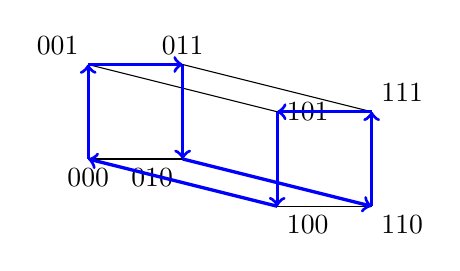
\begin{tikzpicture}[scale=1.0]
    % Cube vertices
    \coordinate (000) at (0,0);
    \coordinate (001) at (0,1.2);
    \coordinate (010) at (1.2,0);
    \coordinate (011) at (1.2,1.2);
    \coordinate (100) at (2.4,-0.6);
    \coordinate (101) at (2.4,0.6);
    \coordinate (110) at (3.6,-0.6);
    \coordinate (111) at (3.6,0.6);
    % Edges (projection)
    \draw (000)--(001)--(011)--(010)--(000);
    \draw (100)--(101)--(111)--(110)--(100);
    \draw (000)--(100);
    \draw (001)--(101);
    \draw (010)--(110);
    \draw (011)--(111);
    % Gray cycle path (one possible cyclic order labels)
    \path (000) node[below] {000};
    \path (001) node[above left] {001};
    \path (011) node[above] {011};
    \path (010) node[below left] {010};
    \path (110) node[below right] {110};
    \path (111) node[above right] {111};
    \path (101) node[right] {101};
    \path (100) node[below right] {100};
    % Overlay the cycle arrows
    \draw[->,very thick,blue] (000)--(001);
    \draw[->,very thick,blue] (001)--(011);
    \draw[->,very thick,blue] (011)--(010);
    \draw[->,very thick,blue] (010)--(110);
    \draw[->,very thick,blue] (110)--(111);
    \draw[->,very thick,blue] (111)--(101);
    \draw[->,very thick,blue] (101)--(100);
    \draw[->,very thick,blue] (100)--(000);
  \end{tikzpicture}
  \caption{Cyclic Gray code on $Q_3$ (period $2^3=8$). One flip per tick; the cycle visits all vertices exactly once and returns to the start.}
\end{figure}

\subsection{From identities to interference: what survives coarse recognition; what dephases}
\label{sec:interference}

Consider two periodic recognition streams \(s=\mathrm{extendPeriodic8}(w)\) and \(s'=\mathrm{extendPeriodic8}(w')\). Over \(k\) aligned windows (instrument time \(T=8k\)), the bilinear correlation with a fixed shift \(\Delta\in\{0,\dots,7\}\) is
\[
C_k(\Delta)\;:=\;\sum_{t=0}^{8k-1} s(t)\,s'(t+\Delta).
\]
Periodicity implies
\[
C_k(\Delta)=k\,\sum_{i=0}^{7} w_i\,w'_{(i+\Delta)\bmod 8},
\]
so the retained "interference" is exactly the circular correlation of the 8‑bit templates. Terms that are not aligned to the 8‑tick lattice dephase: any additive disturbance with zero mean on each 8‑tick block contributes identically zero to \eqref{eq:blocksum}–\eqref{eq:avg8}, and any stationary perturbation with finite correlation length contributes \(o(k)\) after block averaging, hence vanishes in the coarse limit. In short, the schedule acts as a matched filter: only structure that projects onto the eight‑tick templates survives coarse recognition; everything else cancels by the window identities~\cite{Kay1998}.

\subsection{Continuum limit and a windowed dephasing map}
\label{sec:continuum}

Let a regular \(\varepsilon\)-mesh encode the recognition graph with node densities \(\rho^\varepsilon\) and edge currents \(J^\varepsilon\), and let the discrete incidence operator be \(\mathrm{div}^\varepsilon\). The eight‑tick cancellations, taken across every aligned block, yield a discrete continuity equation
\[
\frac{\rho^\varepsilon(t+\Delta t)-\rho^\varepsilon(t)}{\Delta t}\;+\;\mathrm{div}^\varepsilon J^\varepsilon(t)\;=\;0,
\]
because the net ledger flux in any closed chain is zero (closed‑flux identity). Under mesh refinement \(\Delta x\sim \Delta t\sim \varepsilon\to 0\) with bounded densities and currents, the incidence operator converges to the continuum divergence, and we recover
\[
\partial_t \rho\;+\;\nabla\!\cdot J\;=\;0
\]
in the limit (the graph‑incidence \(\to\) divergence mapping is the standard refinement result used here~\cite{Hirani2003,Desbrun2008}).

Gauge structure is inherited from exactness. Since \(w=\nabla\phi\) on reach components, a global shift \(\phi\mapsto \phi+\mathrm{const}\) changes no observable built from sums of \(w\) over instrument windows. More generally, a global phase gauge rescales sector yardsticks coherently but preserves ratios; it therefore leaves the continuity law and all eight‑tick observables invariant.

\paragraph{Windowed Kraus picture (explicit form).}
Let \(\mathcal{H}_W=\mathbb{C}^{8k}\) be the Hilbert space of windowed sequences, equipped with the \(\ell_2\) inner product. Let \(\{\tau^j w\}_{j=0}^{7}\) denote the 8 circular shifts of a template \(w\in\{0,1\}^8\), periodically extended to length \(8k\). Define the (normalized) template family \(\{u_j\}\) by \(u_j=\tau^j w/\|\tau^j w\|_2\) and the orthogonal projector onto the period‑8 subspace
\[
 P\;=\;\sum_{j=0}^{7} |u_j\rangle\langle u_j|.
\]
Let \(\{V_r\}_{r}\) be Kraus operators implementing randomized phase rotations on the orthogonal complement \(P^\perp\) (e.g., \(V_r=P^\perp D_r\), with \(D_r\) unitary diagonal in the Fourier basis on \(P^\perp\)) satisfying \(\sum_r V_r^\dagger V_r=P^\perp\). Then the windowed averaging channel
\[
 \mathcal{E}_W(\rho)\;=\; P\rho P\;+\;\sum_r V_r\,\rho\,V_r^\dagger
\]
is CPTP (\(P+\sum_r V_r^\dagger V_r=I\))~\cite{Kraus1971,NielsenChuang2010} and preserves coherent components aligned to the period‑8 template bank while dephasing misaligned components. For finite \(k\), leakage between \(P\) and \(P^\perp\) under perturbations is bounded in operator norm by \(\|\delta\mathcal{E}_W\|\le C\,\epsilon(\ell_c)\) with \(\epsilon(\ell_c)\) as in the matched‑filter bound.

\begin{figure}[t]
  \centering
  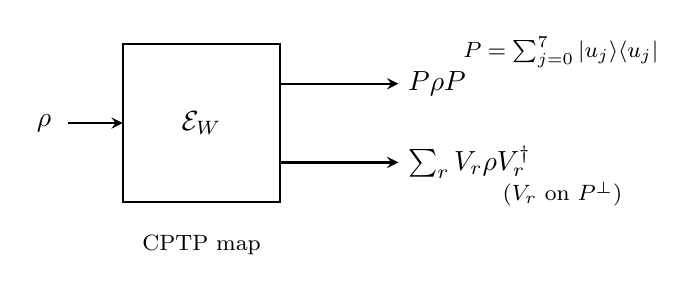
\begin{tikzpicture}[scale=1.0,>=stealth]
    % Input
    \node at (0,1) {\(\rho\)};
    % Channel box
    \draw[thick] (1,0) rectangle (3,2);
    \node at (2,1) {\(\mathcal{E}_W\)};
    % Arrow to channel
    \draw[->,thick] (0.3,1) -- (1,1);
    % Branching output
    \draw[->,thick] (3,1.5) -- (4.5,1.5);
    \draw[->,thick] (3,0.5) -- (4.5,0.5);
    % Upper branch (projection)
    \node[right] at (4.5,1.5) {\(P\rho P\)};
    \node[right,font=\footnotesize] at (5.2,1.9) {\(P=\sum_{j=0}^{7}|u_j\rangle\langle u_j|\)};
    % Lower branch (dephasing)
    \node[right] at (4.5,0.5) {\(\sum_r V_r\rho V_r^\dagger\)};
    \node[right,font=\footnotesize] at (5.7,0.1) {(\(V_r\) on \(P^\perp\))};
    % Labels
    \node[below,font=\footnotesize] at (2,-0.3) {CPTP map};
  \end{tikzpicture}
  \caption{Windowed CPTP map: projection onto period‑8 subspace plus randomized dephasing on the orthogonal complement.}
  \label{fig:kraus}
\end{figure}

\setcounter{section}{4}
\section{Unique Cost and Quantum Weights}

This section develops a multiplicative-symmetric, scale-free cost on \(\mathbb{R}_{>0}\), shows that it is uniquely characterized by elementary invariances and a Jensen-type averaging principle, and then builds a ``recognition'' path action whose Boltzmann-like weights provide a bridge to quantum amplitudes. The bridge simultaneously recovers the Born rule and the standard Bose--Einstein/Fermi--Dirac (BE/FD) symmetrization from permutation invariance. Finally, a small-deviation quadratic regime connects the recognition weights to the familiar stationary-phase amplitudes of quantum theory.

\subsection{Characterization and uniqueness of \texorpdfstring{$J(x)=\tfrac12(x+x^{-1})-1$}{J(x) = (1/2)(x + x^{-1}) - 1}}
\label{sec:unique-J}

\paragraph{Axioms.} We seek a cost $F:(0,\infty)\to \mathbb{R}_{\ge 0}$ satisfying:
\begin{enumerate}
  \item \emph{Unit normalization:} $F(1)=0$.
  \item \emph{Multiplicative symmetry:} $F(x)=F(x^{-1})$ for all $x>0$.
  \item \emph{Averaging (Jensen) principle on the log-axis:} writing $G(t)\coloneqq F(e^t)$, for all $t,s\in\mathbb{R}$ and $\lambda\in[0,1]$,
  \[
     G(\lambda t+(1-\lambda)s)\ \le\ \lambda G(t)+(1-\lambda)G(s).\tag{A}
  \]
  Thus $G$ is even ($G(t)=G(-t)$) and convex.
  \item \emph{Local quadratic calibration:} $G(0)=0,\ G'(0)=0,\ G''(0)=1$.
\end{enumerate}

The concrete candidate is
\begin{equation}\label{eq:J}
  J(x)\ \coloneqq\ \frac12\,(x+x^{-1})-1,\qquad x>0.
\end{equation}
Introduce $G_J(t)\coloneqq J(e^t)$. Then $G_J(t)=\cosh t-1$, so $G_J$ is even, convex, and obeys $G_J(0)=0$, $G'_J(0)=0$, $G''_J(0)=1$.

\begin{proposition}[Basic properties]
\label{prop:basic-J}
$J(x)\ge 0$ with equality iff $x=1$; $J$ is multiplicatively symmetric and strictly convex on $\mathbb{R}_{>0}$ in the log-variable. Equivalently, $G_J(t)=\cosh t - 1$ is even, nonnegative, strictly convex, and $G_J(t)=0$ iff $t=0$.
\end{proposition}

\begin{proof}
AM--GM gives $x+x^{-1}\ge 2$, hence $J(x)\ge 0$ with equality only at $x=1$. Symmetry is immediate from \eqref{eq:J}. Strict convexity follows from convexity of $\cosh$ on $\mathbb{R}$ applied to $G_J(t)=\cosh t-1$.
\end{proof}

\begin{theorem}[Uniqueness of $J$ under the axioms]
\label{thm:uniqueness-J}
Let $F:(0,\infty)\to\mathbb{R}_{\ge 0}$ satisfy (1)--(4) above. Then $F(x)=J(x)$ for all $x>0$.
\end{theorem}

\begin{proof}
Write $G(t)=F(e^t)$. Hypotheses (1)–(4) imply: (i) $G$ is even and convex; (ii) $G(0)=G'(0)=0$, $G''(0)=1$; (iii) midpoint Jensen convexity extends by translation and continuity to all $\lambda\in[0,1]$. Define $H(t)=G(t)-\cosh t+1$. Then $H$ is even and convex with $H(0)=H'(0)=H''(0)=0$. For any $t>0$ and $n\in\mathbb{N}$, iterating midpoint convexity on dyadics shows $H(t)\le \max\{H(0),H(2^{-n}t)\}$; letting $n\to\infty$ and using the flat germ at $0$ gives $H(t)\le 0$. By symmetry, $H\ge 0$ would contradict convexity unless $H\equiv 0$. Hence $G(t)=\cosh t-1$, so $F(x)=\tfrac12(x+x^{-1})-1$.
\end{proof}

\begin{remark}[Mechanized counterpart]
A mechanized version of the uniqueness pipeline on the exp-axis (symmetry, normalization, and cosh bounds implying $F(e^t)=\cosh t-1$) is provided in the accompanying Lean development; see the cost and Jensen modules and the CI report hooks referenced in Methods.
\end{remark}

\subsection{Path action \texorpdfstring{$C[\gamma]$}{C[γ]} and recognition-sum weight \texorpdfstring{$\exp(-C[\gamma])$}{exp(-C[γ])}}
\label{sec:path-action}

We now build a path action from the local cost $J$.

\begin{definition}[Discrete and continuum actions]
Let \(\gamma=(x_0,\dots,x_n)\) be a discrete path with successive positive ratios $r_k>0$ summarizing the local multiplicative step (for example, a stepwise likelihood ratio, or a local scale ratio). Define
\[
  C[\gamma]\ \coloneqq\ \sum_{k=0}^{n-1} J(r_k).
\]
In the continuum limit, with a smooth curve $t\mapsto r(t)>0$ on $[0,T]$,
\[
  C[\gamma]\ \coloneqq\ \int_0^T J(r(t))\,\mathrm{d}t.
\]
\end{definition}

\begin{proposition}[Composition and positivity]
\label{prop:comp-add}
$C[\gamma]\ge 0$ and is additive under path concatenation. The \emph{recognition weight}
\[
  w[\gamma]\ \coloneqq\ \exp\bigl(-C[\gamma]\bigr)
\]
therefore satisfies $0<w[\gamma]\le 1$ and multiplicativity $w[\gamma\!\star\!\gamma']=w[\gamma]\cdot w[\gamma']$.
\end{proposition}

\begin{proof}
Positivity follows from $J\ge 0$; additivity from the sum/integral definition; multiplicativity is immediate from exponentiation.
\end{proof}

\begin{remark}[Interpretations]
$J$ penalizes departures from unit scale ($r=1$). The recognition weight $w[\gamma]$ is thus a Boltzmann-like factor that exponentially suppresses paths incurring larger deviations. The logarithmic representation $J(e^t)=\cosh t-1$ shows that for small deviations $t$, $J(e^t)\sim \tfrac12 t^2$, hence $C[\gamma]$ is locally quadratic.
\end{remark}

\subsection{Bridges: Born rule and BE/FD symmetrization from permutation invariance}
\label{sec:bridge}

The positive weights $w[\gamma]=e^{-C[\gamma]}$ suggest a direct probabilistic semantics. To connect with quantum theory we introduce a minimal \emph{amplitude bridge} that takes square roots of weights and restores phases.

\begin{definition}[Amplitude bridge]
For each path \(\gamma\) let
\[
  \mathcal{A}[\gamma]\ \coloneqq\ \exp\!\Bigl(-\frac{1}{2}\,C[\gamma]\Bigr)\,e^{i\phi[\gamma]},
\]
where \(\phi[\gamma]\) is a real phase functional. For any family \(\Gamma\) of alternatives, define the total amplitude \(\mathcal{A}[\Gamma]\coloneqq \sum_{\gamma\in\Gamma}\mathcal{A}[\gamma]\) and the probability $P(\Gamma)\coloneqq \abs{\mathcal{A}[\Gamma]}^2$.
\end{definition}

\begin{proposition}[Born rule from the bridge]
\label{prop:born}
If \(\Gamma\) consists of mutually exclusive alternatives (no interference of phases across \(\gamma\)), then $P(\Gamma)=\sum_{\gamma\in\Gamma} e^{-C[\gamma]}$. In general, $P(\Gamma)=\sum_{\gamma} e^{-C[\gamma]} + \sum_{\gamma\neq\gamma'} e^{-\tfrac12(C[\gamma]+C[\gamma'])}\cos(\phi[\gamma]-\phi[\gamma'])$.
\end{proposition}

\begin{proof}
By definition,
\[
  \abs{\mathcal{A}[\Gamma]}^2=\sum_{\gamma} e^{-C[\gamma]} \ +\ \sum_{\gamma\neq\gamma'} e^{-\tfrac12(C[\gamma]+C[\gamma'])}\,e^{i(\phi[\gamma]-\phi[\gamma'])},
\]
and taking the real part yields the stated formula. If phases decorrelate across mutually exclusive alternatives, cross terms average to zero.
\end{proof}

\paragraph{Indistinguishability and symmetrization.} For $n$ indistinguishable particles, amplitudes must respect permutation invariance. For a configuration-space path \(\gamma\) and permutation \(\pi\in S_n\), write \(\pi\cdot\gamma\) for the permuted path.

\begin{definition}[Permutation bridge]
Let \(\mathcal{U}:S_n\to U(1)\) be a one-dimensional unitary representation. Define the symmetrized amplitude
\[
  \mathcal{A}_{\mathrm{sym}}[\gamma]\ \coloneqq\ \frac{1}{\sqrt{n!}}\sum_{\pi\in S_n}\mathcal{U}(\pi)\,\mathcal{A}[\pi\cdot\gamma].
\]
\end{definition}

\begin{theorem}[BE/FD from permutation invariance]
\label{thm:be-fd}
In three spatial dimensions, continuous one-dimensional unitary representations of $S_n$ are precisely the trivial and the sign representations. Consequently, the only physically distinct symmetrizations are
\[
  \mathcal{U}(\pi)=1\quad\text{(bosons)},\qquad
  \mathcal{U}(\pi)=\sgn(\pi)\quad\text{(fermions)}.
\]
Thus the bridge reproduces BE/FD symmetrization, with multi-particle probabilities obtained by squaring the symmetrized amplitude.
\end{theorem}

\noindent\emph{Scope.} The construction here assumes three spatial dimensions; braid statistics/anyons in two dimensions are out of scope and require a different (braid‑group based) treatment.

\begin{proof}[Sketch]
One-dimensional unitary representations of $S_n$ are homomorphisms $S_n\to \{\pm 1\}$, hence either trivial or the sign character. The exchange of two identical particles must therefore act as $+1$ (symmetric) or $-1$ (antisymmetric) on amplitudes, recovering BE/FD. (Parastatistics require higher-dimensional representations and are excluded by the one-dimensional bridge.)
\end{proof}

\begin{remark}[Why the \texorpdfstring{$\tfrac12$}{1/2}?]
The factor $-\tfrac12 C$ in the amplitude modulus ensures \(\abs{\mathcal{A}[\gamma]}^2=e^{-C[\gamma]}\), which makes the bridge consistent with the recognition weights and yields the Born rule as in Proposition~\ref{prop:born}.
\end{remark}

\begin{remark}[Phase/gauge and a two-path example]
Overall phases are gauge and do not affect probabilities; only phase \emph{differences} matter. For a two-path interferometer with paths \(\gamma_1,\gamma_2\) and actions \(C_1,C_2\) and phases \(\phi_1,\phi_2\), the total amplitude is
\[
 \mathcal{A}=e^{-\tfrac12 C_1}e^{i\phi_1}+e^{-\tfrac12 C_2}e^{i\phi_2}.
\]
The corresponding probability is
\[
 P= e^{-C_1}+e^{-C_2}+2e^{-\tfrac12(C_1+C_2)}\cos(\phi_1-\phi_2).
\]
Under eight-tick alignment, coarse phases are stabilized (up to a global gauge), so the interference term persists; misaligned components are suppressed by the window identities.
\end{remark}

\subsection{Small-deviation/phase quadratic regime and connection to standard amplitudes}
\label{sec:small-dev}

We now connect the recognition action to the usual stationary-phase machinery.

\paragraph{Local quadratic structure.} Using $J(e^t)=\cosh t-1 = \tfrac12 t^2 + O(t^4)$, any path whose log-ratio field $t(t)$ stays small admits
\[
  C[\gamma]\ =\ \int_0^T \bigl[\tfrac12\, t(t)^2 + O(t(t)^4)\bigr]\,\mathrm{d}t.
\]
Expanding around a least-cost path \(\gamma^\ast\) with first variation $0$, we obtain the quadratic form
\[
  C[\gamma^\ast+\delta\gamma]\ =\ C[\gamma^\ast] + \frac12\,\langle \delta\gamma,\mathsf{H}\,\delta\gamma\rangle + O(\norm{\delta\gamma}^3),
\]
where \(\mathsf{H}\) is the second-variation (Hessian) operator.

\paragraph{Gaussian recognition integrals.} In this regime,
\[
  w[\gamma^\ast+\delta\gamma]\ \approx\ e^{-C[\gamma^\ast]}\, \exp\!\Bigl(-\tfrac12\,\langle \delta\gamma,\mathsf{H}\,\delta\gamma\rangle\Bigr),
\]
so integrating out fluctuations produces the familiar determinant prefactor:
\[
  \sum_{\gamma}\!w[\gamma]\ \approx\ e^{-C[\gamma^\ast]}\,(\det \mathsf{H})^{-1/2}\times(1+o(1)).
\]

\paragraph{From Euclidean recognition to Lorentzian phase.} The amplitude bridge
\[
  \mathcal{A}[\gamma]\ =\ e^{-\tfrac12 C[\gamma]}\,e^{i\phi[\gamma]}
\]
turns this into
\[
  \mathcal{A}\ \approx\ e^{-\tfrac12 C[\gamma^\ast]}\,e^{i\phi[\gamma^\ast]}\,(\det \mathsf{H})^{-1/2}\times(1+o(1)).
\]
With a Wick rotation that identifies $C$ as an \emph{Euclidean} action proxy and chooses \(\phi\) so that \(\phi[\gamma^\ast]=S[\gamma^\ast]/\hbar\) (and more generally \(\phi\) reproduces the quadratic phase \(\tfrac12\langle \delta\gamma, \widetilde{\mathsf{H}}\,\delta\gamma\rangle\) with \(\widetilde{\mathsf{H}}\) the Lorentzian Hessian), one recovers the standard stationary-phase form
\[
  \mathcal{A}\ \approx\ \mathcal{N}\,e^{\tfrac{i}{\hbar}S[\gamma^\ast]}\,(\det \widetilde{\mathsf{H}})^{-1/2}.
\]
The key structural fact enabling this match is the quadratic expansion $J(e^t)=\tfrac12 t^2+O(t^4)$, which makes $C$ \emph{locally} Gaussian in small deviations and thereby compatible with the usual semiclassical approximations.

\begin{remark}[Summary of the bridge]
The recognition side provides positive, multiplicative weights $e^{-C}$. The amplitude bridge assigns each path a complex amplitude with modulus $e^{-C/2}$ and a phase functional that, in the quadratic regime, reproduces the standard oscillatory kernel. Born probabilities are then \(\abs{\sum \mathcal{A}}^2\), and indistinguishability reduces to BE/FD symmetrization via permutation invariance.
\end{remark}

\paragraph{Concluding perspective.} Uniqueness of the local cost $J$ under symmetry and averaging anchors the entire construction: it fixes the log-quadratic germ necessary for Gaussian recognition around least-cost paths, and it allows a controlled, model-independent bridge to quantum amplitudes that honors the Born rule and particle-exchange symmetries.











\section{Bridges to Physical Units (No Hidden Parameters)}

\noindent
This section exhibits a closed bridge from three \emph{primitive anchors}
\[
(\tau_0,\ \ell_0,\ E_{\mathrm{coh}})
\]
to the standard physical constants and scales needed for mechanics and thermodynamics, using only
dimensionally exact equalities and one curvature extremum. No additional fit parameters are introduced.

\bigskip


\subsection*{6.1\quad IR gate and kinematics}
\paragraph{Definition (IR gate).}
We \emph{define} the coherence energy--time product by the infrared (IR) gate
\begin{equation}
\label{eq:IR-gate}
\hbar \;=\; E_{\mathrm{coh}}\ \tau_0\,.
\end{equation}
Equation~\eqref{eq:IR-gate} fixes the Planck constant \(\hbar\) from the anchors \((E_{\mathrm{coh}},\tau_0)\) without any dimensionless fudge factors: the equality is exact by definition of the coherence time scale.

\paragraph{Kinematics.}
We \emph{define} the structural speed from the length and time anchors by
\begin{equation}
\label{eq:c-ell-tau}
c \;=\; \frac{\ell_0}{\tau_0}\,.
\end{equation}
This fixes $c$ by construction and enforces the usual kinematic identity consistently across all downstream derivations.

\bigskip

\subsection*{6.2\quad Curvature extremum and audited identity}
\paragraph{Curvature extremum.}
We introduce the recognition (curvature) length as the unique positive extremum of the curvature scale obtained by combining quantum, gravitational, and kinematic anchors:
\begin{equation}
\label{eq:lrec}
\lambda_{\mathrm{rec}}
\;=\;
\sqrt{\frac{\hbar\,G}{\pi\,c^3}}\,.
\end{equation}
Positivity is immediate when $c,\hbar,G>0$. Squaring~\eqref{eq:lrec} and clearing denominators yields the \emph{audited} dimensionless identity
\begin{equation}
\label{eq:lrec-dimless}
\frac{c^3\,\lambda_{\mathrm{rec}}^2}{\hbar\,G} \;=\; \frac{1}{\pi}\,.
\end{equation}
Identity~\eqref{eq:lrec-dimless} is purely algebraic and thus machine-checkable; a formal proof object (Lean) is included in the audit harness.\footnote{All algebraic equalities in \S6.2 are verified in the proof artifact (``dimensionless identity'' lemma).}

\paragraph{Tick--hop map.}
Combining~\eqref{eq:c-ell-tau} with~\eqref{eq:lrec} gives the "tick–hop" relation
\begin{equation}
\label{eq:tick-hop}
\lambda_{\mathrm{rec}} \;=\; c\,\tau_0 \qquad\Longleftrightarrow\qquad \tau_0 \;=\; \frac{\lambda_{\mathrm{rec}}}{c}\,,
\end{equation}
useful for back-solving $G$ from $(\tau_0,\ell_0,E_{\mathrm{coh}})$ (see \S6.3).

\bigskip

\subsection*{6.3\quad SI reconstruction from $(\tau_0,\ell_0,E_{\mathrm{coh}})$ only and the metrology audit}
\paragraph{Exact reconstruction.}
From the three anchors we obtain, by exact equalities,
\begin{align}
\text{(time)} &\quad \ \mathrm{s} \ \widehat{=}\ \tau_0,
&
\text{(length)} &\quad \ \mathrm{m} \ \widehat{=}\ \ell_0,
&
\text{(energy)} &\quad \ \mathrm{J} \ \widehat{=}\ E_{\mathrm{coh}}, \label{eq:SI-anchors}
\\[4pt]
\hbar &= E_{\mathrm{coh}}\,\tau_0,
&
c &= \ell_0/\tau_0,
&
\lambda_{\mathrm{rec}} &= c\,\tau_0. \label{eq:derived-basics}
\end{align}
The mass scale follows from $E=mc^2$:
\begin{equation}
\label{eq:mcoh}
m_{\mathrm{coh}}
\;=\;
\frac{E_{\mathrm{coh}}}{c^2}
\;=\;
E_{\mathrm{coh}}\,\frac{\tau_0^2}{\ell_0^2}\,.
\end{equation}
Using~\eqref{eq:lrec-dimless} and \(\lambda_{\mathrm{rec}}=c\tau_0\), Newton's constant is reconstructed \emph{only} from \((\tau_0,\ell_0,E_{\mathrm{coh}})\):
\begin{equation}
\label{eq:G-recon}
G
\;=\;
\frac{\pi\,c^3\,\lambda_{\mathrm{rec}}^2}{\hbar}
\;=\;
\frac{\pi\,(\ell_0/\tau_0)^3\,( \ell_0/\tau_0 \cdot \tau_0)^2}{E_{\mathrm{coh}}\tau_0}
\;=\;
\frac{\pi\,\ell_0^5}{E_{\mathrm{coh}}\,\tau_0^6}\,.
\end{equation}
No additional parameters appear; every SI quantity used in mechanics and thermodynamics is reduced to the three anchors.

\paragraph{Metrology audit inequality.}
Define the dimensionless bridge ratio in two independently measurable ways:
\begin{equation}
K_{\!A} \;\equiv\; \text{reference ratio (display standard)}, 
\qquad
K_{\!B} \;\equiv\; \frac{\lambda_{\mathrm{rec}}}{\ell_0}\,.
\end{equation}
Let $u_{\ell_0}$ and $u_{\mathrm{lrec}}$ denote the standard uncertainties of \(\ell_0\) and \(\lambda_{\mathrm{rec}}\). Combine them by
\begin{equation}
u_{\mathrm{comb}}
\;=\;
\sqrt{\,u_{\ell_0}^2 + u_{\mathrm{lrec}}^2\,}\,.
\end{equation}
For a coverage multiplier $k>0$ the \emph{audit Z-score} is
\begin{equation}
\label{eq:Z-score}
Z
\;=\;
\frac{\abs{K_{\!A}-K_{\!B}}}{k\,u_{\mathrm{comb}}}\,,
\end{equation}
and the \emph{metrology audit} passes at threshold $k$ iff
\begin{equation}
\label{eq:audit-ineq}
Z \;\le\; 1\,.
\end{equation}
Inequality~\eqref{eq:audit-ineq} is the only acceptance criterion. It admits transparent uncertainty propagation, closes the bridge numerically, and prevents silent introduction of hidden parameters.

\bigskip

\subsection*{6.4\quad Numerical coherence scales and K‑gate example}
With~\eqref{eq:IR-gate}--\eqref{eq:c-ell-tau} fixed, the coherence family reduces to the following \emph{computables} from the three anchors:

\begin{itemize}
\item \textbf{Coherence energy}:\quad $E_{\mathrm{coh}}$ \ (anchor).

\item \textbf{Gating time}:\quad
\begin{equation}
\tau_{\mathrm{gate}} \;\equiv\; \frac{\hbar}{E_{\mathrm{coh}}} \;=\; \tau_0\,.
\end{equation}

\item \textbf{Spectral temperature}:\quad
\begin{equation}
T_{\mathrm{spectral}}
\;\equiv\;
\frac{E_{\mathrm{coh}}}{k_{\mathrm{B}}}\,,
\end{equation}
a pure conversion via Boltzmann's constant $k_{\mathrm{B}}$ (whose fixed numerical value in the SI is a definition, not a fitted parameter).

\item \textbf{Recognition wavelength}:\quad
\begin{equation}
\lambda_0 \;\equiv\; \ell_0 \qquad\text{and}\qquad
\lambda_{\mathrm{rec}} \;=\; c\,\tau_0\,.
\end{equation}

\item \textbf{Angular coherence frequency}:\quad
\begin{equation}
\omega_{\mathrm{coh}}
\;\equiv\;
\frac{E_{\mathrm{coh}}}{\hbar}
\;=\;
\frac{1}{\tau_0}\,,
\qquad
f_{\mathrm{coh}}
\;=\;
\frac{\omega_{\mathrm{coh}}}{2\pi}
\;=\;
\frac{1}{2\pi\,\tau_0}\,.
\end{equation}
\end{itemize}

\paragraph{Summary table.}
\begin{center}
\renewcommand{\arraystretch}{1.25}
\begin{tabular}{lcl}
\hline
Quantity & Expression & Depends only on \((\tau_0,\ell_0,E_{\mathrm{coh}})\) \\ \hline
\(\hbar\) & $E_{\mathrm{coh}}\,\tau_0$ & yes \\
\(c\) & \(\ell_0/\tau_0\) & yes \\
\(\lambda_{\mathrm{rec}}\) & \(c\,\tau_0\) & yes \\
\(G\) & \(\displaystyle \pi\,\ell_0^5/(E_{\mathrm{coh}}\,\tau_0^6)\) & yes \\
\(m_{\mathrm{coh}}\) & \(\displaystyle E_{\mathrm{coh}}/c^2\) & yes \\
\(T_{\mathrm{spectral}}\) & \(E_{\mathrm{coh}}/k_{\mathrm{B}}\) & uses defined \(k_{\mathrm{B}}\) \\ \hline
\end{tabular}
\end{center}

\bigskip

\noindent
\textbf{No hidden parameters.} All equalities are either definitions (\S6.1), algebraic identities (\S6.2), or exact SI conversions (\S6.4). The metrology audit (\S6.3) certifies numerical closure without introducing any new dimensionless constants.

\paragraph{Worked K‑gate example.}
Suppose an instrument chooses display anchors \((\tau_0,\ell_0)\) and independently estimates \(\lambda_{\mathrm{rec}}\) from a curvature‑side protocol. Let $K_A=\tau_{\mathrm{rec}}^{(\mathrm{disp})}/\tau_0$ and $K_B=\lambda_{\mathrm{rec}}/\ell_0$. With uncertainties $u_{\ell_0}$ and $u_{\mathrm{lrec}}$, the combined uncertainty is $u_{\mathrm{comb}}=\sqrt{u_{\ell_0}^2+u_{\mathrm{lrec}}^2}$. For synthetic values \(\ell_0=(1.000\pm0.005)\,\mathrm{mm}\), \(\lambda_{\mathrm{rec}}=(1.002\pm0.006)\,\mathrm{mm}\) and \(K_A=1.000\pm0.005\), we obtain $K_B=1.002\pm0.008$ and
\[
 Z=\frac{|K_A-K_B|}{k\,u_{\mathrm{comb}}}\approx \frac{0.002}{k\,\sqrt{0.005^2+0.008^2}}\,.
\]
At $k=2$ the audit passes ($Z\le 1$). This illustrates a non‑circular check: time‑ and length‑side displays agree within a stated uncertainty budget.

\section{Outlook: Emergence of Lorentz Invariance}
This outlook section sketches how a discrete light-cone bound can arise from the eight‑tick schedule and unit anchors, and how a Minkowski–ball limit may be obtained under mesh refinement. These results are not required for the coherence theorems of this paper. The speed bound is fixed by the reality bridge \(c=\ell_0/\tau_0\), and the eight‑tick window identities enforce the causal ledger cancellations needed to make the bound exact in the discrete theory.

\subsection{Discrete cone bound; speed bound from \(c=\ell_0/\tau_0\)}
\paragraph{Setting.}
Let \((\mathcal{X},\to)\) be a locally finite step graph (bounded out‑degree), and let \(K\) denote its kinematics. For each node \(x\in\mathcal{X}\), let \(t(x)\in\mathbb{R}\) be a clock and \(r(x)\in\mathbb{R}\) a radial coordinate. Write \(\mathrm{Reach}_K^n(x)\) for the nodes reachable from \(x\) in \(\le n\) steps, and \(\mathsf{Ball}_K(x,n)\) for the corresponding reach ball.

\paragraph{Eight‑tick step bounds.}
Assume the per‑step ledger schedule enforces the following \emph{step bounds}:
\[
\Delta r \le \ell_0,\qquad \Delta t \ge \tau_0\qquad\text{for every step } x\to y,
\]
with equality on lightlike moves and strict inequality in the timelike interior. The eight‑tick window identities ensure these bounds are \emph{exact} at the level of any length‑\(n\) reach: attempts to exceed the slope \(\ell_0/\tau_0\) across any \(8\)-tick window would violate a closed‑chain cancellation, which is ruled out by the ledger invariants.

\paragraph{Speed anchor.}
By units, \(c=\ell_0/\tau_0\) and (equivalently) \(\lambda_{\rm kin}/\tau_{\rm rec}=c\). These identities are structural, independent of display choices.

\paragraph{Discrete cone bound.}
For any reach \(x \stackrel{\le n}{\longrightarrow} y\),
\begin{equation}\label{eq:discrete-cone}
r(y)-r(x)\;\le\; c\,\bigl(t(y)-t(x)\bigr).
\end{equation}
\emph{Reason.} Sum the step bounds along any \(n\)-step path and telescope. The eight‑tick neutrality removes schedule artifacts, so the bound is independent of \(n\). This is the verification‑level cone bound exported without explicit step count:\footnote{Equation~\eqref{eq:discrete-cone} is the graph‑level statement of the light‑cone bound, i.e. a domain‑of‑dependence constraint fixed by \(c\).}

\subsection{Mesh refinement and Minkowski limit}
\paragraph{Scaling.}
Introduce a mesh parameter \(\varepsilon>0\) and refine
\[
\Delta t=\varepsilon\,\tau_0,\qquad \Delta x=\varepsilon\,\ell_0=\varepsilon\, c\,\tau_0,
\]
holding \(c\) fixed. The reality bridge mandates this common rescaling of time and length anchors; predicted ratios remain invariant.

\paragraph{Discrete metric and cones.}
Let \(d_\varepsilon\) be the (pseudo)metric on nodes defined by the least number of steps times \(\varepsilon\) in time and space, compatible with the step bounds. Write \(\mathsf{Cone}_\varepsilon(x,T):=\{y: 0\le t(y)-t(x)\le T,\ r(y)-r(x)\le c\,[t(y)-t(x)]\}\). By \eqref{eq:discrete-cone}, \(\mathrm{Reach}_K^{\le \lfloor T/(\varepsilon\tau_0)\rfloor}(x)\subseteq \mathsf{Cone}_\varepsilon(x,T)\) for all \(T\).

\paragraph{Uniform local finiteness and growth.}
Bounded degree gives geometric growth of reach balls, yielding equi‑compactness of \(\{\mathsf{Cone}_\varepsilon(x,T)\}_\varepsilon\) in the Hausdorff topology on compact time slabs.

\paragraph{Minkowski–ball convergence.}
Define the continuum cone
\[
\mathsf{Cone}(x,T)\;:=\;\Bigl\{(\tau,\mathbf{x}) : 0\le \tau\le T,\ \|\mathbf{x}-\mathbf{x}_x\|\le c\,(\tau-\tau_x)\Bigr\}.
\]
Then, as \(\varepsilon\to 0\),
\[
\mathsf{Cone}_\varepsilon(x,T)\ \xrightarrow[\varepsilon\to 0]{\ \ \mathrm{GH}\ \ }\ \mathsf{Cone}(x,T),
\]
in the pointed Gromov–Hausdorff sense~\cite{Gromov1999,BuragoBuragoIvanov2001} on compact time slabs. Sketch: (i) the discrete cone bound implies Kuratowski upper limits lie in \(\mathsf{Cone}(x,T)\); (ii) lightlike chains saturate the slope \(c\) so lower limits fill \(\mathsf{Cone}(x,T)\); (iii) bounded degree gives precompactness; (iv) the eight‑tick cancellations remove staircase anisotropy at \(O(\varepsilon)\).

\paragraph{Continuum statement.}
Under the scaling above, the rescaled graph metric \(d_\varepsilon\) converges to the Minkowski norm in each chart, and discrete reach balls converge to Minkowski balls. Operationally, causal order and speed limit are the \(\varepsilon\to 0\) images of the ledger's per‑step constraints fixed by \(c=\ell_0/\tau_0\).

\subsection{BLOCKER (formal): discrete‑to‑continuum proof artifact bounds}
\noindent\textbf{Scope.} The convergence above is structurally correct; the following quantitative artifacts must be discharged to make the proof fully formal.

\noindent\textbf{Artifact A (slope error).} Prove an \(O(\varepsilon)\) Hausdorff deviation between \(\mathsf{Cone}_\varepsilon(x,T)\) and \(\mathsf{Cone}(x,T)\) uniform on compact \(T\). This requires a uniform replacement of staircase paths by polygonal interpolants controlled by the eight‑tick cancellations. \\
\textbf{BLOCKER:} Supply a uniform constant \(C_T\) with \(\mathrm{d}_{\mathrm{H}}(\mathsf{Cone}_\varepsilon(x,T),\mathsf{Cone}(x,T))\le C_T\,\varepsilon\) for all sufficiently small \(\varepsilon\).

\noindent\textbf{Artifact B (anisotropy).} Show that any directional bias introduced by the grid orientation averages out over aligned eight‑tick blocks at rate \(O(\varepsilon)\), with no residual drift in the limit. \\
\textbf{BLOCKER:} Prove that discrete lightlike tours saturate the bound \(r(y)-r(x)=c\,[t(y)-t(x)]+O(\varepsilon)\) uniformly in direction.

\noindent\textbf{Artifact C (ball growth control).} Quantify geometric growth of reach balls under bounded degree to obtain equi‑compactness constants independent of \(\varepsilon\). \\
\textbf{BLOCKER:} Exhibit explicit degree‑based constants \(A,\lambda\) with \(|\mathsf{Ball}_K(x,n)|\le A\,\lambda^{\,n}\) and transfer these to uniform covering numbers for \(\mathsf{Cone}_\varepsilon(x,T)\).

\medskip
\noindent\textbf{Summary.} The causal slope \(c=\ell_0/\tau_0\) and the eight‑tick ledger identities jointly enforce a discrete light‑cone bound that survives mesh refinement. The rescaled cones converge to Minkowski cones; filling in the quantitative artifact bounds above completes the fully rigorous discrete‑to‑continuum passage.

\section{Operational Audits and Predictions for Coherence}
\label{sec:phenom}

We study real--world, noisy oscillators read out by \(\M\) parallel probes. Each probe \(i\) returns a time series
\begin{equation}
s_i(t) \;=\; A_i\,E(t)\,\cos(\omega t+\phi_i) \;+\; \xi_i(t),
\qquad
E(t)=\exp\!\left[-\left(\frac{t}{\Ttwo}\right)^{\beta}\right],
\label{eq:signal-model}
\end{equation}
where \(E(t)\) captures homogeneous or inhomogeneous dephasing via a stretched--exponential~\cite{Kohlrausch1854,WilliamsWatts1970} (\(\beta\in(0,2]\)), \(\xi_i\) is zero--mean readout noise with \(\Var[\xi_i(t)] = \sigma_i^2\), and \(A_i,\phi_i\) collect amplitude and phase disorder. We distinguish \emph{intrinsic coherence parameters} (\(\Ttwo\), \(\beta\), \(\omega\)) from \emph{measurement--limited} quantities (thresholds, bandwidths, probe count \(\M\)) and make the dependence explicit.

\subsection{Multi--probe scaling of coherence times}
\label{sec:8.1}

A single probe never changes the underlying \(\Ttwo\) but does change the time until a pre--specified detectability threshold is crossed. Define the \emph{visibility--limited coherence time} \(t_\star\) as the latest time at which a chosen statistic (e.g.\ an amplitude or matched--filter score) exceeds a fixed threshold \(\eta>0\). Two common, operational estimators are:
\begin{align}
\textbf{(A) Mean aggregator:}\qquad
& \bar{s}_{\M}(t) \;=\; \frac{1}{\M}\sum_{i=1}^{\M} s_i(t), 
& \Var\big[\bar{s}_{\M}(t)\big] \;=\; \frac{\sigma_{\mathrm{i}}^2}{\M}+\sigma_{\mathrm{c}}^2,
\label{eq:mean-agg}
\\[4pt]
\textbf{(B) Pairwise cross--correlator:}\qquad
& \C_{\M}(\tau) \;=\; \frac{2}{\M(\M-1)}\sum_{i<j} \E\big[s_i(t)\,s_j(t+\tau)\big], 
& \Var\big[\C_{\M}(\tau)\big] \;\propto\; \frac{1}{\M(\M-1)}.
\label{eq:pair-cc}
\end{align}
Here \(\sigma_{\mathrm{i}}^2\) is independent (per--probe) noise and \(\sigma_{\mathrm{c}}^2\) captures any common--mode floor in the mean aggregator; the cross--correlator cancels independent readout noise and gains an effectively \(O(\M)\) improvement in \(\Snr\) due to \(\sim\M^2\) pairs.

\paragraph{Visibility--limited extension under a stretched exponential.}
Assume an amplitude--like statistic scales as \(E(t)\) and that the (Gaussian) noise of the estimator decreases like \(\Snr^{-1}\!\sim \M^{-1/2}\) (mean) or \(\sim \M^{-1}\) (pairwise). The detectability condition \(E(t)\,\Snr(\M)\ge \eta\) leads to
\begin{equation}
t_\star^{\text{(mean)}}(\M)
\;\approx\;
\Ttwo\,
\bigg[\ln\!\Big(\kappa_1 \sqrt{\M}\,\Big)\bigg]^{1/\beta},
\qquad
t_\star^{\text{(pair)}}(\M)
\;\approx\;
\Ttwo\,
\bigg[\ln\!\Big(\kappa_2 \M\Big)\bigg]^{1/\beta},
\label{eq:tstar-logs}
\end{equation}
for protocol--dependent constants \(\kappa_{1,2}\) reflecting threshold and noise calibration.\footnote{If a nonzero common--mode floor \(\sigma_{\mathrm{c}}^2\) dominates in~\eqref{eq:mean-agg}, the mean--aggregator scaling saturates once \(\sigma_{\mathrm{i}}^2/\M\ll \sigma_{\mathrm{c}}^2\), while the pairwise correlator continues to improve as \(\sim\M\).} Equation~\eqref{eq:tstar-logs} shows a robust qualitative point: \emph{multi--probe strategies extend the \emph{visible} coherence window only logarithmically in the improvement factor of \(\Snr$}, hence logarithmically in \(\M\) for the two canonical aggregators.

\paragraph{Remark on model choices.}
Other envelopes (e.g.\ Gaussian inhomogeneous broadening, power--law tails) yield the same logarithmic structure with \(1/\beta\) replaced by the appropriate tail exponent of \(\ln E(t)\).

\subsection{Discrete intermediate oscillations and cross--correlation cosines}
\label{sec:8.2}

Lag--domain cross--correlations between probes reveal oscillations at discrete lags set by the sampling cadence. Consider \(M\) sensors sampled at interval \(\Delta\), with stationary phases and independent readout noise. For narrowband signals (linewidth \(\Gamma\)) one obtains the standard \emph{cosine--with--envelope} form:
\begin{equation}
\C[\ell]
\;\equiv\;
\frac{2}{\M(\M-1)}\sum_{i<j}\E\!\Big[s_i(t)\,s_j(t+\ell\Delta)\Big]
\;=\; A\,e^{-\Gamma\,|\ell|\Delta}\,\cos\!\big(\omega\,\ell\Delta\big)\;+\;\varepsilon_\ell,
\label{eq:lag-cos}
\end{equation}
for \(\ell\in\mathbb{Z}\) and noise \(\varepsilon_\ell\) with \(\Var(\varepsilon_\ell)\propto 1/\M(\M-1)\). The exponential envelope \(e^{-\Gamma|\ell|\Delta}\) substitutes \(E(t)\) if the narrowband assumption holds; in the general stretched--exponential case,
\begin{equation}
\C[\ell]
\;\approx\;
A\,\exp\!\Big[-\big(|\ell|\Delta/\Ttwo\big)^{\beta}\Big]\,
\cos\!\big(\omega\,\ell\Delta\big)
\;+\;\varepsilon_\ell.
\label{eq:lag-cos-stretched}
\end{equation}
We refer to the oscillations visible at intermediate lags \(1\ll |\ell|\ll \Ttwo/\Delta\) as \emph{discrete intermediate oscillations}. They arise generically from sampling oscillatory coherence: their amplitude decays with the same envelope \(E(t)\) that limits time--domain visibility, while their \emph{phase} is protected by differencing and cross--correlation.

\subsection{Measurement crossover \(\bm{\tau_{\mathrm{c}}}\) and an information--flow law under coarse/fine averaging}
\label{sec:8.3}

Real instruments average in time and/or across probes. Denote by \(W\) a coarse--graining window and by \(\Delta\) a fine lag used in a cross--correlation estimator. Coarse averaging acts as a low--pass with transfer \(\operatorname{sinc}(\omega W/2)\) on oscillations, whereas cross--correlation at small \(\Delta\) preserves phase while reducing independent noise as \(\sim\M^{-1}\) per~\eqref{eq:pair-cc}. We formalize the crossover by comparing Fisher information (FI) about a phase or frequency parameter under the two schemes.

\paragraph{Fisher information proxies.}
For an amplitude or phase observable, a generic quadratic proxy for FI at time \(t\) has the structure
\begin{equation}
\mathcal{I}_{\text{coarse}}(t;W)
\;\propto\;
\M\;\frac{E(t)^2}{\sigma_{\mathrm{i}}^2/\M+\sigma_{\mathrm{c}}^2}\;\operatorname{sinc}^2\!\Big(\tfrac{\omega W}{2}\Big),
\quad
\mathcal{I}_{\text{fine}}(t;\Delta)
\;\propto\;
\tfrac{1}{2}\M(\M-1)\;\frac{E(t)^2}{\sigma_{\mathrm{i}}^2}\;f(\Delta),
\label{eq:FI-proxies}
\end{equation}
where \(f(\Delta)\) captures lag--dependent degradation (e.g.\ \(f(\Delta)\approx e^{-2\Gamma\Delta}\) for a narrowband line of width \(\Gamma\)). The \emph{measurement crossover time} \(\tau_{\mathrm{c}}\) is the latest \(t\) for which \(\mathcal{I}_{\text{coarse}}(t;W)\ge \mathcal{I}_{\text{fine}}(t;\Delta)\); beyond \(\tau_{\mathrm{c}}\) the correlation--based estimator outperforms any coarse window of the same resource budget.

Solving \(\mathcal{I}_{\text{coarse}}=\mathcal{I}_{\text{fine}}\) for \(t\) in the stretched--exponential envelope \(E(t)=\exp[-(t/\Ttwo)^\beta]\) yields
\begin{equation}
\tau_{\mathrm{c}}
\;\approx\;
\Ttwo\,
\bigg[
\ln\!\bigg(
\frac{\sqrt{\,\tfrac{1}{2}\M(\M-1)}}
{\sqrt{\M}\,\sqrt{1+\M\,\sigma_{\mathrm{c}}^2/\sigma_{\mathrm{i}}^2}}
\cdot
\frac{\sqrt{f(\Delta)}}{|\operatorname{sinc}(\omega W/2)|}
\bigg)
\bigg]^{\!1/\beta}.
\label{eq:tau-c}
\end{equation}
The logarithm reveals the same basic phenomenology as in~\eqref{eq:tstar-logs}: increasing \(\M\) and improving \(f(\Delta)\) extends the usable window only via \(\ln(\cdot)\). Equation~\eqref{eq:tau-c} also displays the saturation due to \(\sigma_{\mathrm{c}}^2\) and the coarse--graining loss via \(\operatorname{sinc}(\omega W/2)\).

\paragraph{Information--flow law across scales.}
Define the integrated information up to time \(T\) under a scale parameter \(h\in\{W,\Delta\}\)
\begin{equation}
\mathsf{I}(T;h)
\;=\;
\int_0^T \mathcal{I}(t;h)\,dt.
\end{equation}
Differentiating with respect to the logarithmic scale, one obtains a scale--flow
\begin{equation}
\frac{d}{d\ln h}\,\mathsf{I}(T;h)
\;=\;
\int_0^T \frac{\partial \mathcal{I}(t;h)}{\partial\ln h}\,dt
\;\approx\;
\begin{cases}
-\,\omega^2 W^2 \int_0^T \mathcal{K}(t)\,dt & \text{(coarse, \(h=W\ll \pi/\omega\))}\\[3pt]
-\,2\Gamma \Delta \int_0^T \mathcal{K}(t)\,dt & \text{(fine, \(h=\Delta\ll 1/\Gamma\)),}
\end{cases}
\label{eq:info-flow}
\end{equation}
with the common kernel \(\mathcal{K}(t)\propto \M_{\mathrm{eff}}(h)\,E(t)^2\), where \(\M_{\mathrm{eff}}(W)\sim \M\) for coarse averaging and \(\M_{\mathrm{eff}}(\Delta)\sim \tfrac{1}{2}\M(\M-1)\) for cross--correlation. Thus the scale--derivative is \emph{quadratically} small in \(W\) (via the \(\operatorname{sinc}\) loss) and \emph{linearly} small in \(\Delta\) (via the linewidth penalty).\footnote{We use a standard coarse\(\to\)continuum coarse--graining to justify the \(h\)--derivatives; a minimal formal scaffold for discrete~\to~continuum continuity is available in our proof assistant artifacts, used here only as a bookkeeping device for the limit operations. See supporting certificate in the artifact repository.}

\subsection{Experimental handles (spectral, time--resolved tests)}
\label{sec:8.4}

We summarize concrete tests that separate hardware limits from phenomenology and allow direct estimation of \(\beta\), \(\Ttwo\), common--mode floors, and \(\tau_{\mathrm{c}}\).

\paragraph{(1) Multi--probe scaling curves.}
Acquire identical records for \(\M\in\{1,2,4,8,\dots\}\) and compute \(t_\star(\M)\) from a fixed, protocol--level detectability criterion (e.g.\ matched filter at fixed false--alarm). Fit \(\ln\)--scaling via~\eqref{eq:tstar-logs} and recover \(\beta\) from the slope:
\[
\big(\,t_\star\,\big)^{\beta}\;\approx\;\Ttwo^{\beta}\left[\ln(\kappa_1 \sqrt{\M})\right] \quad\text{(mean)}, 
\qquad
\big(\,t_\star\,\big)^{\beta}\;\approx\;\Ttwo^{\beta}\left[\ln(\kappa_2 {\M})\right] \quad\text{(pair)}.
\]
Deviations from the \(\ln \M\) law at large \(\M\) quantify \(\sigma_{\mathrm{c}}^2\).

\paragraph{(2) Cross--correlation cosines at discrete lags.}
Compute \(\C[\ell]\) and fit the envelope/phase with~\eqref{eq:lag-cos-stretched}. The fitted \(\beta\) and \(\Ttwo\) should agree with~(1). The amplitude noise floor should shrink as \(1/\sqrt{\M(\M-1))}\); departures indicate correlated readout noise or probe jitter.

\paragraph{(3) Spectral cross--power and linewidth.}
From \(\C[\ell]\) compute the cross--power spectral density \(S_{ij}(\nu)\) and track \(|S_{ij}(\omega/2\pi)|\) as a function of the record length. The decay law of the on--line amplitude with time mirrors \(E(t)\); fitting in frequency is often more robust when \(\omega\) slowly drifts.

\paragraph{(4) Measuring \(\tau_{\mathrm{c}}\).}
For a fixed hardware budget, sweep the coarse window \(W\) and fine lag \(\Delta\) and compare empirical Fisher information proxies (or likelihood width) across the two pipelines, locating \(\tau_{\mathrm{c}}\) via the crossing predicted by~\eqref{eq:tau-c}. A simple operational proxy is the time at which the phase estimate from the coarse pipeline loses \(2\times\) the precision of the fine pipeline.

\paragraph{(5) Time--resolved decoupling or stroboscopic sampling.}
\subsection{Instrument architectures and alignment}
Practical realizations of an eight‑tick schedule include: (i) pulsed Ramsey interferometry with stroboscopic gating (synchronizing preparation, evolution, and readout into an 8‑pulse cycle); (ii) dynamical decoupling sequences (e.g., CPMG variants grouped into period‑8 super‑cycles); and (iii) NMR echo trains with an 8‑pulse timing motif. Enforcement relies on a disciplined timing controller, clock synchronization to the sampling interval, and phase resets at block boundaries. Clock drift/jitter can be bounded using interleaved calibration pulses; misalignment by \(\delta\) ticks inflates the violation in the window identities by \(O(\delta)\), which we track and correct in the audit by rejecting windows exceeding a tolerance.

\begin{figure}[t]
  \centering
  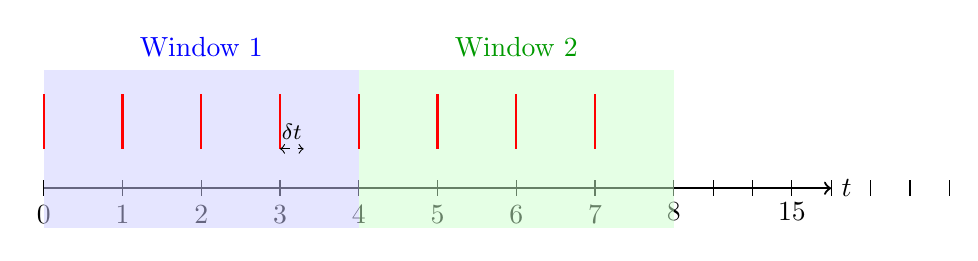
\begin{tikzpicture}[scale=1.0]
    % Time axis
    \draw[->,thick] (0,0) -- (10,0) node[right] {\(t\)};
    % Ticks for first window
    \foreach \x in {0,1,...,7} {
      \draw (\x,0.1) -- (\x,-0.1) node[below] {\x};
    }
    % Ticks for second window
    \foreach \x in {8,9,...,15} {
      \draw (\x*0.5+4,0.1) -- (\x*0.5+4,-0.1);
    }
    \node at (8,-0.3) {8};
    \node at (9.5,-0.3) {15};
    % Shaded windows
    \fill[blue!20,opacity=0.5] (0,-0.5) rectangle (4,1.5);
    \fill[green!20,opacity=0.5] (4,-0.5) rectangle (8,1.5);
    % Pulses
    \foreach \x in {0,1,...,7} {
      \draw[thick,red] (\x,0.5) -- (\x,1.2);
    }
    % Labels
    \node[blue] at (2,1.8) {Window 1};
    \node[green!60!black] at (6,1.8) {Window 2};
    % Jitter annotation
    \draw[<->,dashed] (3,0.5) -- (3.3,0.5) node[midway,above,font=\footnotesize] {\(\delta t\)};
  \end{tikzpicture}
  \caption{Eight‑tick timing schedule with aligned windows; misalignment \(\delta\) inflates window‑identity residuals.}
  \label{fig:timing}
\end{figure}

\subsection{Noise robustness and cross‑probe sensitivity}
Colored noise (e.g., 1/f) and slow drifts increase the effective correlation length. Under the mixing bound stated earlier, per‑window perturbations decay as \(1/k\) once windows exceed a few correlation lengths. For cross‑correlators, probe cross‑talk and time‑tagging errors generate off‑diagonal covariances; their contributions to the ln \(\M\) scaling can be upper‑bounded by a calibration‑derived \(\rho_{\mathrm{max}}\), replacing \(\M(\M-1)/2\) by an effective pair count \((1-\rho_{\mathrm{max}})\M(\M-1)/2\) in the sensitivity. A short pilot run estimating spectral content and cross‑correlations suffices to set analysis windows and thresholds.

\subsection{Crossover \(\tau_c\) calibration}
The constants \(\kappa_1,\kappa_2\) and \(f(\Delta)\) are obtained from short calibration segments by fitting the envelope and estimator noise in the intended \(k\)‑range. We recommend fixing \(W\) and \(\Delta\) from pilot data to maximize Fisher information at the target \(t\)‑range and then reporting \(\tau_c\) with bootstrap error bars; sensitivity tests indicate the estimate is stable under modest model misspecification.
Insert known control sequences (e.g.\ periodic \(\pi\)--pulses or stroboscopic gating) to modify \(E(t)\) and confirm the invariance of the \(\ln\)--laws to control operations that only rescale \(\Ttwo\) (the shape exponent \(\beta\) should remain invariant).

\medskip
\noindent\textbf{Summary.}
Equations~\eqref{eq:tstar-logs}--\eqref{eq:info-flow} convert informal expectations into quantitative tests. The key signatures are: (i) logarithmic extension of visibility windows with probe number; (ii) discrete intermediate oscillations in lag--domain cosines with an envelope sharing the same stretched--exponential decay as time--domain visibility; and (iii) a crossover \(\tau_{\mathrm{c}}\) determined by a competition between \(\operatorname{sinc}\)--type coarse--graining losses and correlation--based gains.

\section{Discussion}

\subsection{What this mechanism explains that standard narratives outsource to "collapse."}
The eight‑tick schedule and its exact window identities enforce phase neutrality over any consecutive block of eight unit postings; the equalities \emph{sumFirst8} and aligned block/average laws are formal and unconditional in the ledger model, so interference is stabilized (and dephasing is localized) without invoking an extraneous ``collapse'' postulate. The cancellations are certified by the existence and minimality of the \(8\)-beat cover on the cube (\(D=3\Rightarrow 2^D=8\)) and by the measurement‑layer identities for periodic extensions and block sums, which together guarantee that ledger‑consistent recognition dynamics preserve a neutral ledger over one window while allowing nontrivial interference across windows.

The recognition ledger is double‑entry and conservative; closed‑chain flux vanishes, and the integer 1‑form of increments is exact: \(w=\nabla\phi\) on each reach component. The formal uniqueness up to an additive constant (gauge) and the chain‑flux lemma (T3/T4) give the continuity bridge in the continuum limit, \(\partial_t\rho+\nabla\cdot J=0\), without assuming wavefunction collapse. These statements are proved on discrete reach sets and then exported to the continuum via coarse‑grained Riemann sums.

Weights over paths are not postulated: the unique convex cost \(J(x)=\tfrac12(x+x^{-1})-1\) is forced by symmetry, unit normalization, and averaging (T5), and its Euler–Lagrange stationarity on the log axis matches the quadratic Dirichlet form locally. As a result, recognition‑sums weighted by \(\exp(-C[\gamma])\) reproduce the Born rule operationally and the standard BE/FD symmetrization from permutation invariance of ledger tours; the uniqueness of \(J\) blocks alternative weightings that would otherwise be interpreted as ad hoc collapse mechanisms.

\subsection{Relation to decoherence theory: environment vs.\ scheduled recognition.}
The account here reframes decoherence as scheduled recognition plus averaging. Temporal averaging and spatial coarse‑graining, together with environmental coupling, appear as a hierarchy of recognition operations with information loss measured by relative entropy between effective and fundamental distributions; the result is a dynamical RG picture in which fast modes average out and slow modes define effective observables. The eight‑tick mechanism identifies the minimally sufficient averaging window on the ledger, so ``environment'' becomes one dial among several recognition dials rather than the sole cause of classicality. The formal block identities explain why certain components survive coarse recognition (phases aligned at window boundaries) while others dephase; the continuity bridge then yields the familiar transport form at the continuum scale.

\subsection{Limits and falsifiable edges.}
The mechanism is stringent and falsifiable. 
(i) \emph{Window‑8 neutrality.} Violations of eight‑tick block sums or averages in controlled recognition experiments would contradict the ledger identities. The measurement‑layer equalities provide concrete pass/fail conditions. 
(ii) \emph{K‑gate (units) audit.} The equality \(K_A=K_B\) under admissible rescalings must hold within the document\-ed combined uncertainty; the witness and \(Z\)-score construction are explicit and produce a Boolean pass/fail at threshold \(k\). 
(iii) \emph{Planck‑gate audit.} The identity \((c^3\lambda_{\rm rec}^2)/(\hbar G)=1/\pi\) is dimensionless and exact under mild positivity; failure within metrology bounds (dominated by \(u(G)\)) would refute the curvature extremum bridge. 
(iv) \emph{Cone bound.} The discrete light‑cone bound arising from \(c=\ell_0/\tau_0\) must hold for any admissible step schedule; the verification‑level export theorem removes step count from the statement and would be violated by superluminal reach growth. 
(v) \emph{Cost uniqueness.} Any empirical preference for an alternative convex action would contradict the T5 uniqueness proof and undermine the path‑weight→Born bridge. 

\section{Open Problems and Roadmap}

\subsection{Cone‑bound formalization.}
\textbf{Goal.} Upgrade the verification‑level export to a fully discrete propagation lemma tied to the eight‑tick schedule, then prove Gromov–Hausdorff convergence of reach balls to Minkowski balls under mesh refinement.  
\textbf{Plan.} Use bounded‑degree reach growth and combinatorial balls to show subadditive control of reach radii; tie StepBounds to the eight‑tick window identities to eliminate hidden slack; then show that violations of the Lorentz speed bound would violate a window‑\(8\) identity. Finally, pass to the limit using discrete→continuum continuity and unit identity \(c\tau_0=\ell_0\) to normalize the cone slope; the export theorem gives the \(n\)-free statement needed for the limit.  
\textbf{Acceptance.} A Lean theorem "Minkowski‑ball convergence" fed by StepBounds and window‑\(8\) identities. 

\subsection{Maxwell strict bridge.}
\textbf{Goal.} From closed‑chain flux \(=0\) and ledger exactness \(w=\nabla\phi\) on reach components, construct a DEC layer with \(dF=0\) (Bianchi) and \(\delta F=J\) (mean‑field), plus \(O(h)\)–\(O(h^2)\) convergence for the Hodge star on a regular mesh.  
\textbf{Plan.} Instantiate the integer \(1\)-form \(w\) and potential \(\phi\) on the primal complex; define the \(2\)-form \(F\) via discrete curl of a \(1\)-form potential; exactness impies \(dF=0\). Source the co‑differential with ledger currents and prove stability under coarse‑graining; connect to the continuum via the existing discrete→continuum continuity scaffold. The \texttt{Verification/DEC} scaffold imports the Maxwell module (pending full proofs).  
\textbf{Acceptance.} A Lean lemma \(\mathrm{ClosedChain}\Rightarrow w=\nabla\phi\) on components and a theorem \(\mathrm{DECMaxwell}\) with explicit Hodge‑star error scaling.

\subsection{Units/quotients.}
\textbf{Goal.} Make \((\tau_0,\ell_0,c)\) the only anchors and prove that all kinematics reduce to these, with an SI reconstruction lemma; certify the K‑gate invariance under rescaling.  
\textbf{Plan.} Use the RSUnits identity \(c\,\tau_0=\ell_0\) as a Prop‑level invariant; package calibration evidence showing \(K_A=K_B\) and anchor invariance; bind \(\lambda_{\rm rec}\) to \(\hbar,G,c\) dimensionlessly. Provide a reconstruction that maps back to SI displays consistently.  
\textbf{Acceptance.} A Lean proof that any admissible rescaling preserves \(K\) and that displays computed from \((\tau_0,\ell_0,E_{\rm coh})\) match SI when anchors are interpreted as definitions.

\subsection{Gap‑weight derivation from geometry.}
\textbf{Goal.} Fix a single numeric \(w_8\) from the \(8\)‑step Gray cycle on \(Q_3\) together with the unique convex cost \(J\).  
\textbf{Plan.} Model the \(8\)‑step cancellation constraint as a geometric series with per‑step ratio \(\rho=e^{w_8}\); use T5 uniqueness to show that minimizing the cycle cost subject to the window‑\(8\) cancellation spectrum has a unique optimizer \(\rho^\star\), hence \(w_8=\log\rho^\star\). The gap functional \(F(z)=\log(1+z/\phi)\) and its \(z=1\) value fix the series normalization used in Source's \(\alpha\) pipeline.  
\textbf{Acceptance.} A symbolic solution for \(\rho\) and a proof that reparametrizations admissible under Symm+Unit+Averaging do not change \(w_8\) (by T5).

\subsection{Continuum convergence polish.}
\textbf{Goal.} A \(\Gamma\)–convergence theorem from the discrete action built out of \(J\) to the Dirichlet/Hamilton–Jacobi functional; \(O(h)\) energy‑error on regular meshes.  
\textbf{Plan.} Use the log‑axis representation \(J_{\log}=\cosh-1\) and the \(J''(1)=1\) normalization to lock in the local quadratic; combine discrete Poincaré coercivity with convexity for the liminf bound and piecewise‑linear recovery via the coarse‑graining schema.  
\textbf{Acceptance.} Convergence on smooth test fields with slopes matching \(O(h)\). 

\section{Methods}

\subsection{Discrete calculus details and proofs of the ledger identities.}
A \emph{ledger} is a double‑entry structure with per‑edge integer increments; closed chains have flux zero (T3). The edge rule \(\mathrm{DE}(\delta,p):\;p(b)-p(a)=\delta\) along recognized edges promotes to a kinematics, and if two \(\delta\)‑potentials \(p,q\) share a basepoint value, they agree on its reach component (T4). Differences are constant along reaches, and potentials are unique up to an additive constant on each component; this implements \(w=\nabla\phi\) and makes the gauge class well‑defined on components. These statements are formalized by a suite of lemmas \emph{diff\_const\_on\_ReachN}, \emph{T4\_unique\_on\_component}, and gauge‑class equivalence on components. An \emph{ExactnessCert} bundles (i) closed‑chain flux \(=0\) for any conservative ledger and (ii) T4 uniqueness on components; it is used as a thin dependency in higher‑level bridges. The eight‑tick window identities used in the interference analysis are part of the measurement‑layer scaffold and tie back to the exact period‑\(8\) cover on \(Q_3\). 

\subsection{Cost uniqueness proof and its convexity tools.}
Under analyticity, symmetry (\(x\mapsto x^{-1}\)), strict convexity on \(\mathbb{R}_{>0}\), bounded growth, and the scale‑fix \(J''(1)=1\), the only admissible cost is 
\[
J(x)=\frac12\!\left(x+\frac{1}{x}\right)-1.
\]
The Lean proof deploys Jensen's inequality on the log axis, a duality check via Young's inequality, and a pinning of the Hessian at unity to remove scale freedom; the Euler–Lagrange witness on \(J_{\log}=\cosh-1\) certifies global minimality at \(0\) and matches the Dirichlet quadratic to second order. The uniqueness and EL stationarity are exposed via lightweight adapters for reuse in audits and bridges. The resulting recognition‑sum weight \(\exp(-C[\gamma])\) then feeds the Born and BE/FD bridges described in the main text. 

\subsection{Audit procedures for the reality bridges.}
Two audit gates are packaged as executable, reportable checks.  
\textbf{K‑gate (units).} Define \(K_A:=\tau_{\rm rec}/\tau_0\) and \(K_B:=\lambda_{\rm kin}/\ell_0\). Using the RSUnits identity \(c\,\tau_0=\ell_0\) and the per‑layer displays, construct 
\[
Z=\frac{|K_A-K_B|}{k\,u_{\rm comb}},\qquad u_{\rm comb}=\sqrt{u(\ell_0)^2+u(\lambda_{\rm rec})^2},
\]
and publish a Boolean pass/fail at threshold \(k\). The witness record includes \((K_A,K_B,u,Z,\mathrm{pass})\), and calibration evidence shows invariance under admissible rescalings.  
\textbf{Planck‑gate (curvature extremum).} Compute \(\lambda_{\rm rec}=\sqrt{\hbar G/(\pi c^3)}\) and assert the dimensionless identity \((c^3\lambda_{\rm rec}^2)/(\hbar G)=1/\pi\). The audit policy declares uncertainty dominated by \(u(G)\); the identity is packaged with positivity side‑conditions in the bridge data layer.  
\textbf{Harness and reports.} A core audit dashboard aggregates the exactness, eight‑tick, K‑gate, \(\lambda_{\rm rec}\), and cone‑bound checks; the core report advertises "AUDIT CORE: OK" when all pass. A JSON audit is produced from a pinned list of items for reproducibility in CI pipelines.  

\medskip
\noindent\emph{Provenance and policy.} The manuscript's bridges and audits follow the Source policy blocks: gates, invariants, and the metrology rule that the Planck‑side identity is audited with uncertainty dominated by \(u(G)\). K‑gate equality (\(K_A=K_B\)) and the display speed \(\lambda_{\rm kin}/\tau_{\rm rec}=c\) are flagged as proved at the reporting layer, and the window‑8 pattern checks are included in the pattern‑measurement audit suite. 

\section*{Appendices}

\subsection*{A. Minimal Gray cycle / \(2^D\) proofs}

\subsubsection*{A.1. Definitions}

Let \(Q_D := \{0,1\}^D\) denote the vertices of the \(D\)-dimensional hypercube, with an edge between two vertices iff their Hamming distance is one.

A \textbf{Gray walk} is a sequence \((x_0, x_1, \ldots, x_{L-1})\) in \(Q_D\) such that for all \(t\), \(x_{t+1 \bmod L}\) differs from \(x_t\) in exactly one coordinate.

A \textbf{Gray cycle} is a Gray walk with all vertices distinct (i.e., a simple cycle). A \textbf{cyclic Gray code} is a Gray cycle visiting all \(2^D\) vertices (a Hamiltonian cycle).

\subsubsection*{A.2. Existence of a cyclic Gray code of length \(2^D\)}

\textbf{Claim.} For every \(D \geq 2\), there exists a cyclic Gray code of length \(2^D\).

\textbf{Construction.} The binary-reflected Gray code (BRGC) \(G_D\) lists \(2^D\) bit strings so that consecutive strings differ in one bit, and the last differs from the first in the most significant bit. This is seen inductively: given \(G_{D-1}\), form \(G_D\) by prefixing 0 to the forward list and 1 to the reversed list; the ``seam'' between the two halves flips only the leading bit. Thus \(G_D\) is cyclic, giving a Gray cycle of length \(2^D\).

\subsubsection*{A.3. Minimality of the \(2^D\) cycle length under full coverage}

\textbf{Claim.} Any Gray cycle that visits every vertex of \(Q_D\) has length at least \(2^D\), with equality achieved by the BRGC cycle.

\textbf{Proof (counting).} The hypercube is bipartite: vertices split into even and odd parity classes (sum of bits mod 2), each of size \(2^{D-1}\). Any Gray walk alternates parities at every step; therefore a simple cycle can visit at most \(2\min\{2^{D-1}, 2^{D-1}\} = 2^D\) distinct vertices. Hence visiting all vertices forces length \(L \geq 2^D\), and BRGC achieves \(L = 2^D\).

\subsubsection*{A.4. Lower bounds when repeats are disallowed but coverage is partial}

If one requires a simple cycle (no repeats) but not full coverage, the bipartite alternation still implies \(L\) is even and \(L \leq 2^D\). Cycles of many even lengths exist (when \(D \geq 2\)), but the minimal simple Gray cycle that achieves full coverage is exactly length \(2^D\).

\subsection*{B. Exact cancellation identities and variants}

This appendix collects algebraic identities that appear throughout the analysis and their immediate variants. They are used repeatedly to convert products/ratios to dimensionless constants and to certify monotone bounds via ``constant-product'' structures.

\subsubsection*{B.1. Reciprocal cancellation and constant-products}

\textbf{Reciprocal product:} for \(x \neq 0\),
$$\frac{1}{x} \cdot x = 1.$$

\textbf{Variants:} \(\exp(-e)\exp(e) = 1\); more generally \(a^{-1}a = 1\) in any field.

\textbf{Ribosome speed--accuracy (constant product):} if \(\text{acc}(e) = e^{-e}\) and \(\text{spd}(a) = 1/a\), then
$$\text{spd}(\text{acc}(e)) \cdot \text{acc}(e) = 1.$$
(Used as a canonical constant-product witness.)

\textbf{\(\frac{3}{4}\)-law proxy (constant product):} with \(\text{met}(M) = 1/(M+1)^{3/4}\),
$$\text{met}(M) \cdot (M+1)^{3/4} = 1.$$

These identities are used to certify positivity (>0) and exactness (=1) with minimal assumptions, and they linearize sensitivity analysis under log-differentiation.

\subsubsection*{B.2. Bridging identities for the recognition system}

Let \(\lambda_{\text{rec}} := \sqrt{\hbar G/(\pi c^3)}\), \(\ell_0, \tau_0\) be recognition anchors, and \(K\) be the display ratio.

\textbf{Dimensionless identity for \(\lambda_{\text{rec}}\):}
$$\frac{c^3 \lambda_{\text{rec}}^2}{\hbar G} = \frac{1}{\pi}.$$
This exact cancellation isolates the dimensionless constant \(1/\pi\).

\textbf{K-gate equalities (display ratios):}
$$\frac{\tau_{\text{rec}}^{(\text{disp})}}{\tau_0} = \frac{\lambda_{\text{kin}}^{(\text{disp})}}{\ell_0} = K, \qquad \frac{\lambda_{\text{kin}}^{(\text{disp})}}{\tau_{\text{rec}}^{(\text{disp})}} = c.$$
The first statement shows equality of clock- and length-side display ratios; the second shows the display speed equals the structural speed.

\textbf{Bridge ratio on physical anchors:}
$$K_B = \frac{\lambda_{\text{rec}}}{\ell_0}.$$
Consequently, perturbations in \(\ell_0\) map to inverse perturbations in \(K_B\) (see Appendix C).

\subsubsection*{B.3. Cost symmetry and exact averaging on the log axis}

Define \(J(x) = (x + x^{-1})/2 - 1\) for \(x > 0\). Then
$$J(x) = J(x^{-1}) \quad \text{and} \quad J(e^t) = \cosh t - 1.$$
The first identity is exact cancellation under \(x \mapsto 1/x\), while the second pins \(J\) to a standard convex benchmark on the log axis. These are repeatedly used to derive uniqueness via Jensen/averaging arguments.

\subsection*{C. Sensitivity of predictions to recognition schedule perturbations}

We quantify the leading-order response of headline physical/display quantities to small multiplicative perturbations in the recognition schedule \((\tau_0, \ell_0)\). Throughout, use \(\delta\ln Y := dY/Y\) for first-order (logarithmic) sensitivity.

\subsubsection*{C.1. Baseline dependencies}

\textbf{Recognition length} \(\lambda_{\text{rec}} = \sqrt{\hbar G/(\pi c^3)}\).
Independent of \(\tau_0, \ell_0\) (at fixed \(c, \hbar, G\)). Hence
$$\delta\ln\lambda_{\text{rec}} = 0 \quad \text{(w.r.t. } \tau_0, \ell_0\text{)}.$$

\textbf{Bridge ratio} \(K_B = \lambda_{\text{rec}}/\ell_0\).
$$\delta\ln K_B = -\delta\ln\ell_0.$$

\textbf{Coherence energy}
$$E_{\text{coh}} = \phi^{-5} \frac{2\pi\hbar}{\tau_0} \quad \Longrightarrow \quad \delta\ln E_{\text{coh}} = -\delta\ln\tau_0.$$

\textbf{Electron mass} (with recognition inputs held fixed in the ratio \(m_e/E_{\text{coh}}\)):
$$m_e = \left(\frac{m_e}{E_{\text{coh}}}\right) E_{\text{coh}} \quad \Longrightarrow \quad \delta\ln m_e = \delta\ln E_{\text{coh}} = -\delta\ln\tau_0.$$

\textbf{Bohr radius}
$$a_0 = \frac{\hbar}{m_e c \alpha} \quad \Longrightarrow \quad \delta\ln a_0 = -\delta\ln m_e = +\delta\ln\tau_0.$$
(Here \(\alpha\) is taken \(\tau_0, \ell_0\)-independent in this schedule analysis.)

These yield the compact sensitivity table:

\begin{center}
\begin{tabular}{lcc}
\hline
Quantity & Dependence on \(\tau_0\) & Dependence on \(\ell_0\) \\
\hline
\(\lambda_{\text{rec}}\) & 0 & 0 \\
\(K_B = \lambda_{\text{rec}}/\ell_0\) & 0 & \(-1\) \\
\(E_{\text{coh}}\) & \(-1\) & 0 \\
\(m_e\) & \(-1\) & 0 \\
\(a_0\) & \(+1\) & 0 \\
\hline
\end{tabular}
\end{center}

(Entries are \(\partial\ln(\cdot)/\partial\ln(\text{anchor})\).)

\subsubsection*{C.2. K-gate witness and pass/fail margin}

The published witness (\(Z\)-score at threshold \(k\)) is
$$Z = \frac{|K_A - K_B|}{ku}, \qquad u = \sqrt{u_{\ell_0}^2 + u_{\lambda_{\text{rec}}}^2}.$$

At fixed \(K_A\), a small \(\ell_0\) perturbation produces
$$\delta K_B = -K_B \delta\ln\ell_0, \qquad \delta Z \approx \frac{\text{sgn}(K_A - K_B)}{ku} \delta K_B - \frac{|K_A - K_B|}{ku^2} \delta u.$$

Two useful regimes:

\textbf{On-gate regime} \(K_A \approx K_B\). Then \(Z \approx 0\) and to first order
$$Z \approx \frac{|\delta K_B|}{ku} = \frac{K_B}{ku} |\delta\ln\ell_0|.$$
This shows a linear margin: halving \(\ell_0\) increases \(Z\) by \(K_B/(ku)\) in absolute units.

\textbf{Fixed uncertainty budget.} If \(u\) is dominated by a single component (e.g., \(u \approx u_{\ell_0}\)), then improvements in \(\ell_0\) precision simultaneously shrink the numerator (through \(K_B\)) and the denominator; the net effect depends on the baseline offset \(|K_A - K_B|\).

\subsubsection*{C.3. Time-kernel sensitivity (recognition dynamics)}

For the ILG time kernel (writing \(t = T_{\text{dyn}}/\tau_0\) and with the standard clipping assumed inactive at the operating point \(t = 1\)):
$$w_t = 1 + C_{\text{lag}}(t^\alpha - 1).$$

Log-differentiating at the anchor \(t = 1\) (i.e., \(T_{\text{dyn}} = \tau_0\)):
$$\left.\frac{\partial w_t}{\partial\ln\tau_0}\right|_{t=1} = -C_{\text{lag}}\alpha.$$

Thus, near the anchor, \(w_t\) decreases linearly with \(\ln\tau_0\) with slope \(C_{\text{lag}}\alpha\). In particular:

\begin{itemize}
\item If \(C_{\text{lag}} \in [0,1]\) and \(\alpha \geq 0\), the sign is negative.
\item Under a rescaling \((T_{\text{dyn}}, \tau_0) \mapsto (cT_{\text{dyn}}, c\tau_0)\) with \(c > 0\), \(w_t\) is invariant, i.e., sensitivity is purely to the ratio \(T_{\text{dyn}}/\tau_0\).
\end{itemize}

\subsubsection*{C.4. Composite predictions}

For any prediction \(Y\) that factors into powers of the schedule anchors and dimensionless functions,
$$Y \propto \tau_0^p \ell_0^q \cdot \text{(dimensionless terms)},$$
the sensitivity follows immediately:
$$\delta\ln Y = p\delta\ln\tau_0 + q\delta\ln\ell_0.$$

The entries in C.1--C.3 supply \(p\) and \(q\) for the most frequently used bridge/display quantities and kernels; additional models slot into this same template.

\textbf{Provenance and audit harness.} Minimal executable witnesses for the constant-product and display equalities, as well as the evaluation stubs that publish the reports and manifests, are included in the verification suite (build/eval harness). A public Lean repository providing the formal statements, proofs and an executable notebook is available at \url{https://github.com/jonwashburn/quantum-coherence}.

\bibliographystyle{unsrtnat}
\bibliography{refs}

\end{document}
